\documentclass[a4paper,landscape,pdftex]{article}
\usepackage[boldmath,boldtext]{nvefoil}

\Trtitle{Cosmic Rays and Gamma Ray Bursts}
\author{Nick van Eijndhoven}
\date{Brussel, 2019}

\begin{document}

\begin{titlepage}
\begin{center}
\vspace*{-4cm}
\Title[18cm]{yellow}{blue}{Cosmic Rays and Gamma Ray Bursts}
{\LARGE \bf
 Nick van Eijndhoven\\[1mm]
 nick@icecube.wisc.edu $\quad$ http://www.iihe.ac.be\\[2mm]
 \includegraphics[keepaspectratio,height=2cm]{vublogo} $\qquad$
 \includegraphics[keepaspectratio,height=2cm]{iihelogo}\\[3mm]
 Vrije Universiteit Brussel - IIHE(ULB-VUB)\\[1mm]
 Pleinlaan 2, B-1050 Brussel, Belgium
}
\end{center}
\Contscb{yellow}{blue}{Contents}{blue}
\end{titlepage}

\twocolumn

\Transcb{yellow}{blue}{Cosmic rays}
\begin{center}
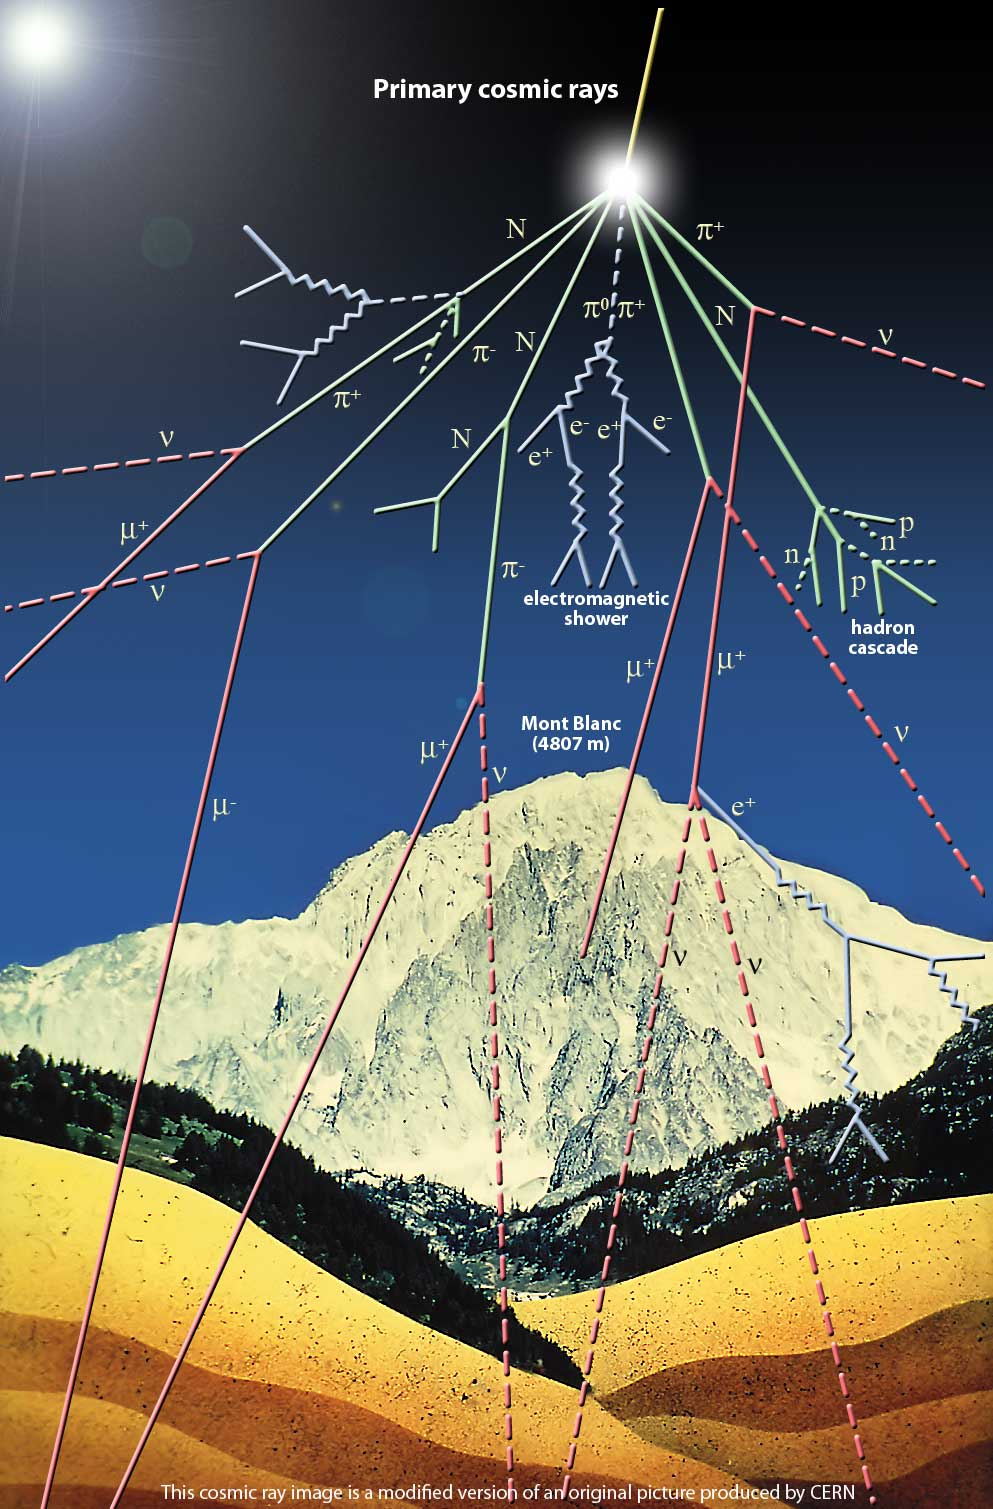
\includegraphics[keepaspectratio,height=15cm]{cosray}
\end{center}

\newpage

\vspace*{1cm}
\begin{itemize}
\item Observations :
\item[] Charge leaks slowly from capacitors
\item[] Effect is smaller when shielded
\item Idea :
\item[] Air gets ionised by charged particles
\item Where do these particles come from ?
\item[] From outer space (Hess 1912)
\item What sort of particles are these ?
\item[] Cosmic ray experiments
\end{itemize}

\Tr
\begin{center}
{\blue Cosmic ray spectra}\\[5mm]
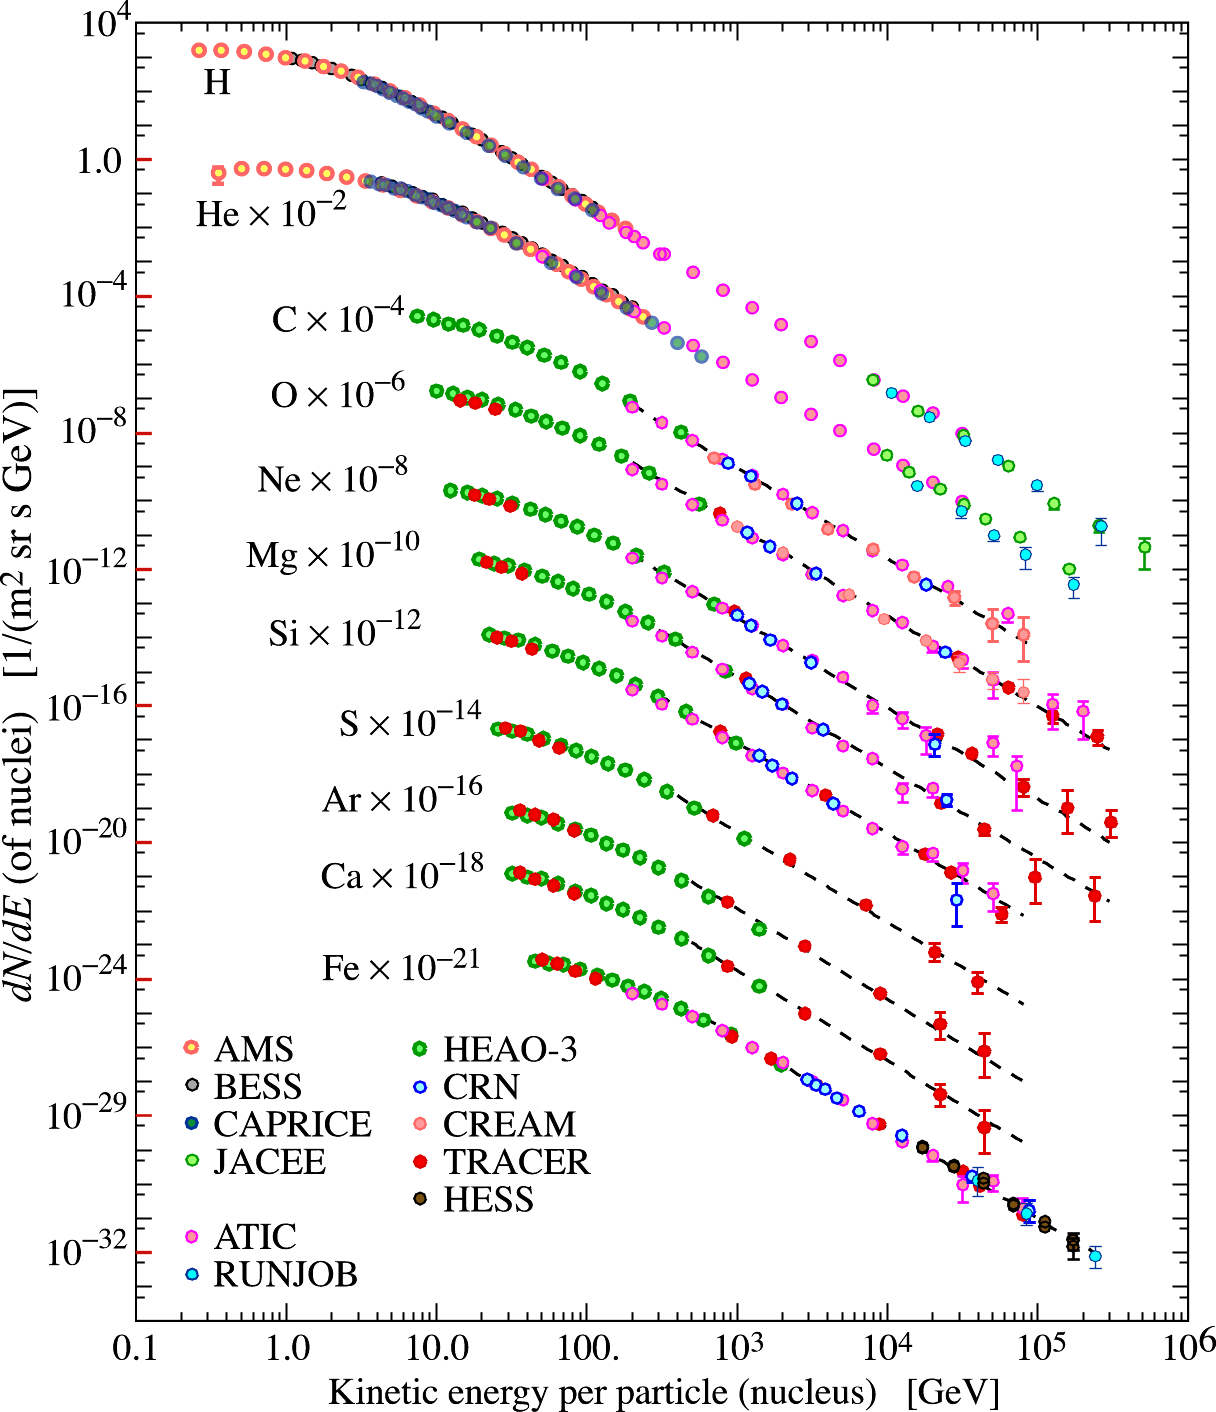
\includegraphics[keepaspectratio,height=13cm]{cr-low-e}
\end{center}

\newpage

\vspace*{1mm}
\begin{itemize}
\item[] Below 10 GeV $\rightarrow$ Solar modulation
\item[] At higher energies we observe
\item Proportions of major components\\
      relatively constant with energy
\item $\frac{\d N}{\d E} \propto E^{-2.6}$
\item Boron spectrum falls steeper
\item[] B is a spallation product of C and O
\item[] Secondary (e.g. spallation) nuclei steeper than primaries
\item sec./prim. decreases as energy increases
\item[] $\rightarrow$ High E rays diffuse out of galaxy faster
\end{itemize}
%
\colorbox{yellow}{What is the maximum energy~?}

\Tr
\vspace*{1.5cm}
\begin{center}
{\blue $E^{2.6}$ scaled flux}\\[5mm]
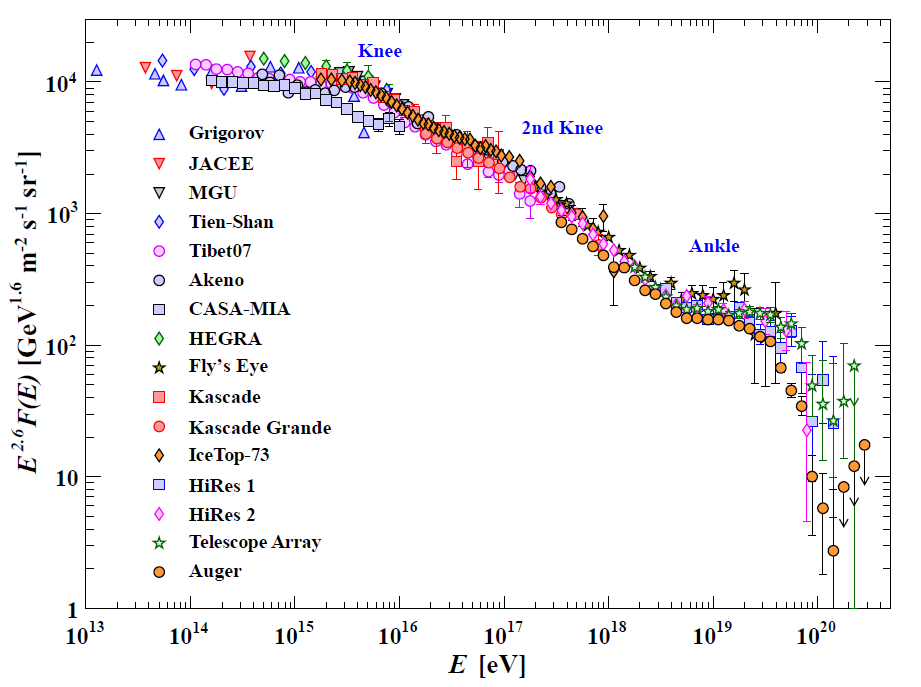
\includegraphics[keepaspectratio,width=13.5cm]{cr-all-scaled26}
\end{center}

\newpage

\vspace*{3cm}
\begin{itemize}
\item Spectral features observed (knee, ankle)
\item[] $E$ limits of different cosmic accelerators~?
\item[] What are these cosmic accelerator sites~?
\item Rather large uncertainties in flux 
\item[] Due to different exp. and models\\
        (see later)
\end{itemize}
%
\colorbox{yellow}{What is the cosmic acceleration mechanism~?}

\Tr
\twocolumn[\begin{center}{\blue Shock wave acceleration}\end{center}]
%
\begin{itemize}
\item Shock front due to an explosive event
\item[] Thin matter sheet with $v>v_{sound}$
\item[] $\rightarrow$ bulk motion ($\Delta v$) after the shock
\item Let a particle enter downstream of the shock
      and pass the front
\item[] {\blue Energy gain $\Delta E=\alpha E \quad (\alpha \propto \Delta v/c)$}
\item[] May backscatter downstream again
\item[] $\rightarrow$ process may be repeated
\item {\blue Multy-step particle acceleration}
\item[] Start energy $E_{0}$ and escape prob. $P_{esc}$
\item[$\ast$] After $n$ encounters~: $E_{n}=E_{0}(1+\alpha)^{n}$
\item[] $\rightarrow n=\frac{\ln(E/E_{0})}{\ln(1+\alpha)}$ to reach energy $E$
\item[] and $P_{stay}(n)=P_{stay}^{n}=(1-P_{esc})^{n}$
\end{itemize}

\newpage

\begin{itemize}
\item Number of particles with energy above $E$
\item[] $\displaystyle N(>E) \propto \sum_{k=n}^{\infty} P_{stay}^{k}
        =\frac{\left(1-P_{esc}\right)^{n}}{P_{esc}}$
\item[] Resulting in a spectrum
\item[] \begin{center}
        {\blue $N(>E) \propto \frac{1}{P_{esc}} \left(\frac{E}{E_{0}}\right)^{-\beta}$}
        \end{center}
\item[] where $\beta=\frac{-\ln(1-P_{esc})}{\ln(1+\alpha)} \approx \frac{P_{esc}}{\alpha}$
\end{itemize}

\begin{center}
\colorbox{yellow}{Indeed a powerlaw spectrum is obtained !}
\end{center}

\begin{itemize}
\item[] Note~: $P_{esc}$ is related to mean free path
\item[] \colorbox{yellow}{Spectral slope $\beta \propto (\sigma \cdot \text{density})^{-1}$}
\item[] {\blue Where do we find shock waves ?}
\end{itemize}

\Tr
\onecolumn
\begin{center}
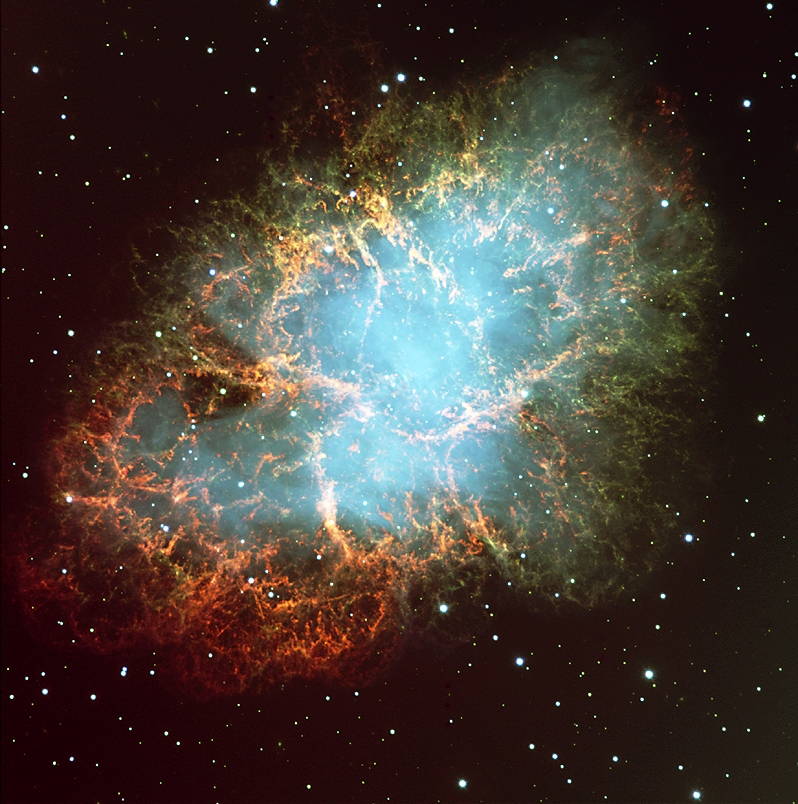
\includegraphics[keepaspectratio,height=15cm]{crab}
\end{center}

\Tr
\begin{center}
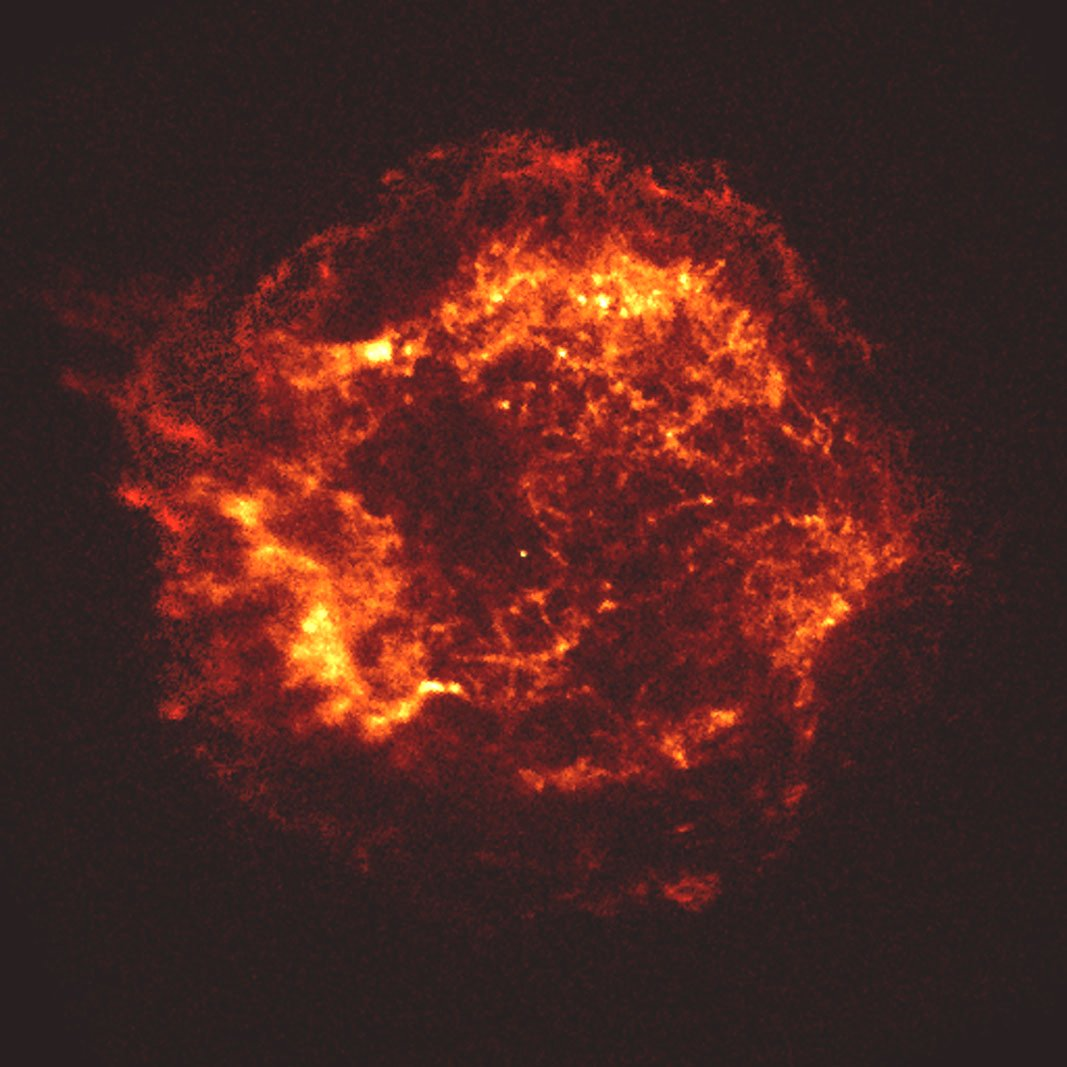
\includegraphics[keepaspectratio,height=15cm]{Cas_A}
\end{center}

\Tr
\twocolumn[\begin{center}{\blue Origin of cosmic rays}\end{center}]
%
\begin{itemize}
\item \colorbox{yellow}{Supernova blast waves}
\item[] Moving charge in static mag. field
\item[] Gyroradius $r=\frac{p}{ZeB} \quad (\vec{p} \perp \vec{B})$
\item[] $\rightarrow
         {\blue \left(\frac{p}{1~\rm{eV}}\right)=0.03 \cdot Z \left(\frac{B}{1~\mu\rm{G}}\right)
         \left(\frac{r}{1~\rm{m}}\right)}$
\item[] Shock wave~: extra factor $(\Gamma\beta)_{shock}$
\item Accelerator of size $R$
\item[] $r > R \rightarrow \text{particles~escape} \rightarrow E_{max}$
\item[] Typical~: $B \approx \mu\text{G} \quad R \approx 3 \cdot 10^{16}$ m
\item[] $\rightarrow$ \colorbox{yellow}{Protons~: $E_{max} \approx 10^{15}$ eV}
\item[$\ast$] At a certain $r \rightarrow {\blue E_{Z}=Z E_{proton}}$
\item[$\ast$] $E>10^{19}~\text{eV} \rightarrow r>R_{galaxy}$
\item[] $\Rightarrow$ Extra-galactic origin
\end{itemize}

\newpage
%
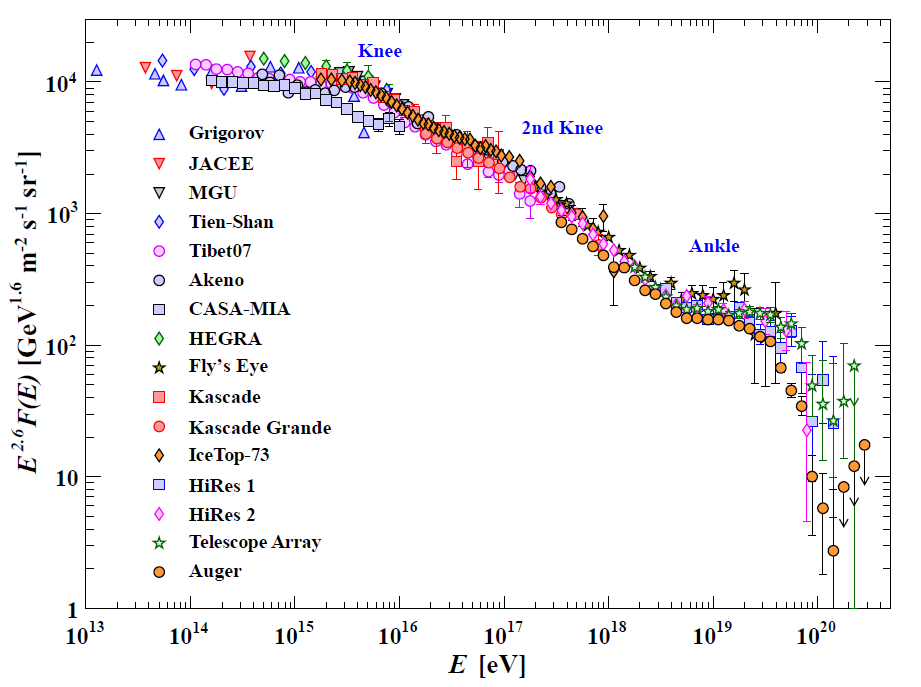
\includegraphics[keepaspectratio,width=12cm]{cr-all-scaled26}
%
\begin{itemize}
\item[] \colorbox{yellow}{What causes the slope change and 'ankle' ?}
\item[] Change in composition ?
\item[] New cosmic sources ?
\item[] \colorbox{yellow}{Do we see the GZK effect above $10^{19}$~eV ?}
\end{itemize}

\Tr
\twocolumn[\begin{center}{\blue Analysis of cosmic ray cascades}\end{center}]
%
\begin{itemize}
\item Only sec. from atm. interactions observed
\begin{itemize}
\item[$\ast$] Properties of shower development
\end{itemize}
\item Multidim. $(N_{e},N_{\mu})$ shower analysis
\begin{enumerate}
\item At prim. vertex~: $\pi$, $K$, $\Lambda$, $\Xi$, $D$, ...
\item At shower maximum~: large $N_{e}$
\item After max.~: meson decays $\rightarrow \mu$, $\nu_{\mu}$
\item Even later~: $\mu$ decays $\rightarrow e$, $\nu_{e}$, $\nu_{\mu}$
\end{enumerate}
\item[] {\blue With increasing primary $E$}
\begin{itemize}
\item[$\ast$] Maximum closer to detector $(D_{max})$
\item[] $D_{max}$ from e.g. fluorescence meas.
\item[$\ast$] Larger sec. energies $\rightarrow$ longer lifetimes
\end{itemize}
\item[] {\blue $\rightarrow N_{e}/N_{\mu}$ increases}
\item[] $N_{e}/N_{\mu} \propto (E/A)^{\alpha} \quad (\alpha > 0)$
\end{itemize}

\newpage

\begin{itemize}
\item $A$ dependence (composition)
\item[] $N_{\mu} \propto (A/E)^{\alpha}\,N_{e}$
\item[] Certain prim. $E$ $\rightarrow N_{\mu} \propto A^{\alpha}\,N_{e}$
\begin{itemize}
\item[$\ast$] {\blue Heavy primaries $\rightarrow$ Muon rich showers}
\item[] Set scale limits by p and Fe
\item[$\ast$] {\blue $N_{e}/N_{\mu}$ (and $D_{max}$) $\rightarrow A \rightarrow E$}
\end{itemize}
\item[] \colorbox{yellow}{Quantitative analysis $\rightarrow$ MC needed}
\item Large discrepancies between various models
\item[] \colorbox{yellow}{Data needed to validate/tune models}
\item[$\ast$] CERN-LHC might provide insight here
\item[] {\blue Physics $E(Z)$ or cascade $E(A)$ effect~?}
\end{itemize}

\Transcb{yellow}{blue}{Possible high-energy sources}
\twocolumn
\begin{center}
{\blue Active Galactic Nuclei (AGN)}\\[1cm]
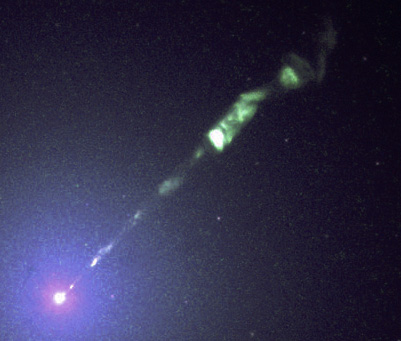
\includegraphics[keepaspectratio,width=13cm]{M87jet}
\end{center}

\newpage

\begin{center}
{\blue Gamma Ray Bursts (GRBs)}\\[1cm]
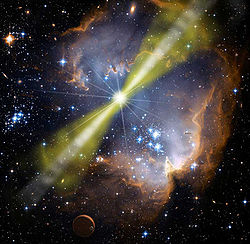
\includegraphics[keepaspectratio,width=6cm]{grb}\\[3mm]
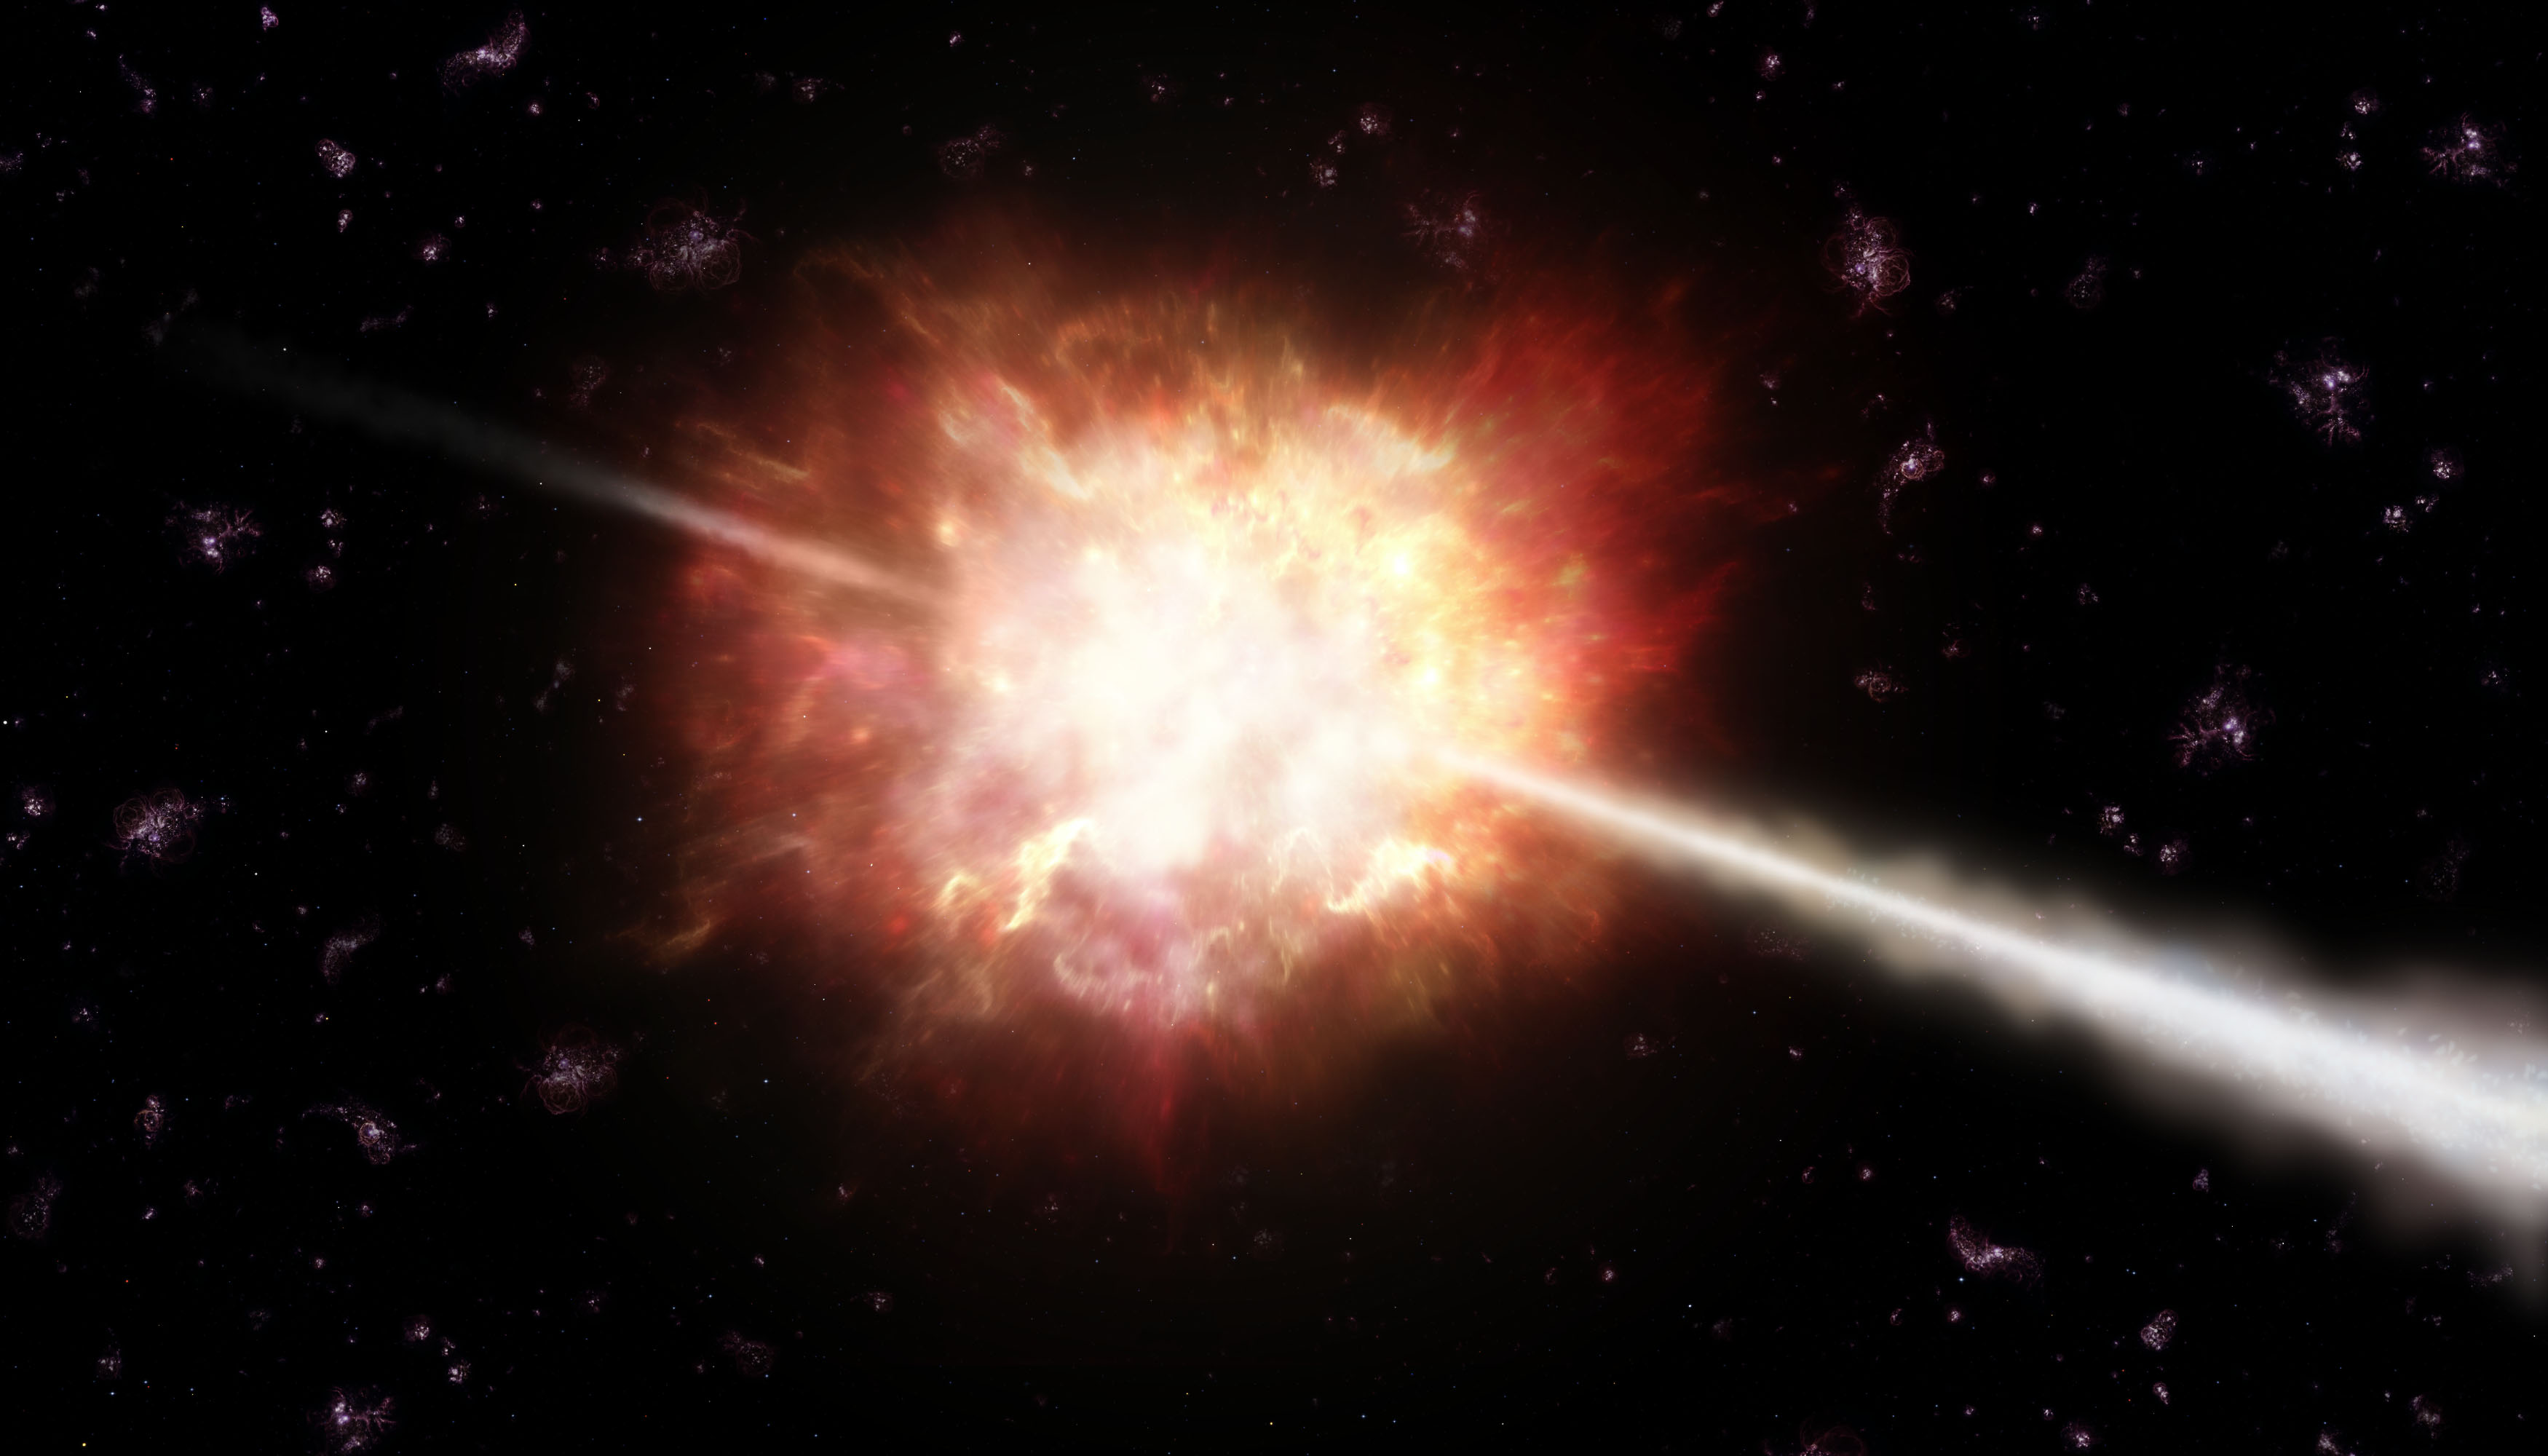
\includegraphics[keepaspectratio,width=12cm]{grb2}
\end{center}

\Tr
\begin{dinglist}{228}
\item Engines which power AGN
\begin{itemize}
\item Acceleration via shock waves in the jets
\item Jet directed to us $\rightarrow$ Blazar
\item[] Markarian 421 and 501
\end{itemize}
\item Gamma Ray Bursts
\begin{itemize}
\item 'Hypernovae' $\rightarrow$ Black hole
\item NS+NS or NS+BH mergers
\item[] {\blue Also shock wave acceleration}
\end{itemize}
\item Cold dark matter (WIMPs, SUSY particles)
\begin{itemize}
\item Annihilation $\rightarrow$ {\blue High $E$ neutrinos}
\item[] {\red WIMPs at the center of Sun, Earth ?}
\end{itemize}
\item[$\ast$] \colorbox{yellow}{Most extreme events are GRBs}
\item[] {\blue Can GRBs produce the flux at the ankle ?}
\item[] Waxman\&Bahcall PRL 78 (1997) 2292
\end{dinglist}

\newpage

\begin{center}
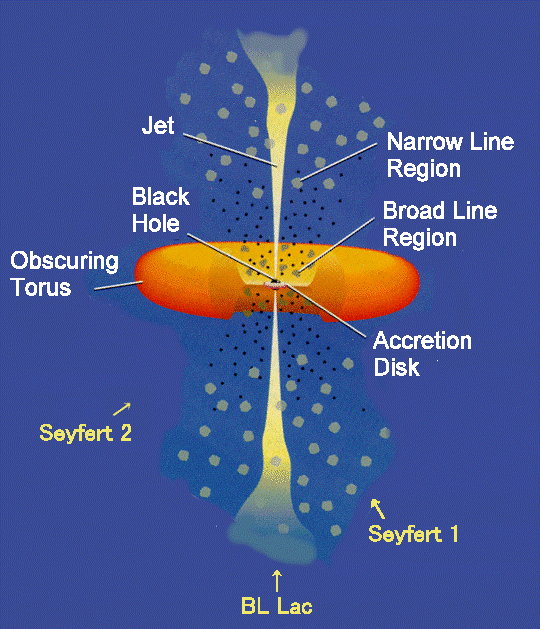
\includegraphics[keepaspectratio,width=13cm]{agn-1}
\end{center}

\Tr
\begin{center}
{\blue Processes in the jet}\\[5mm]
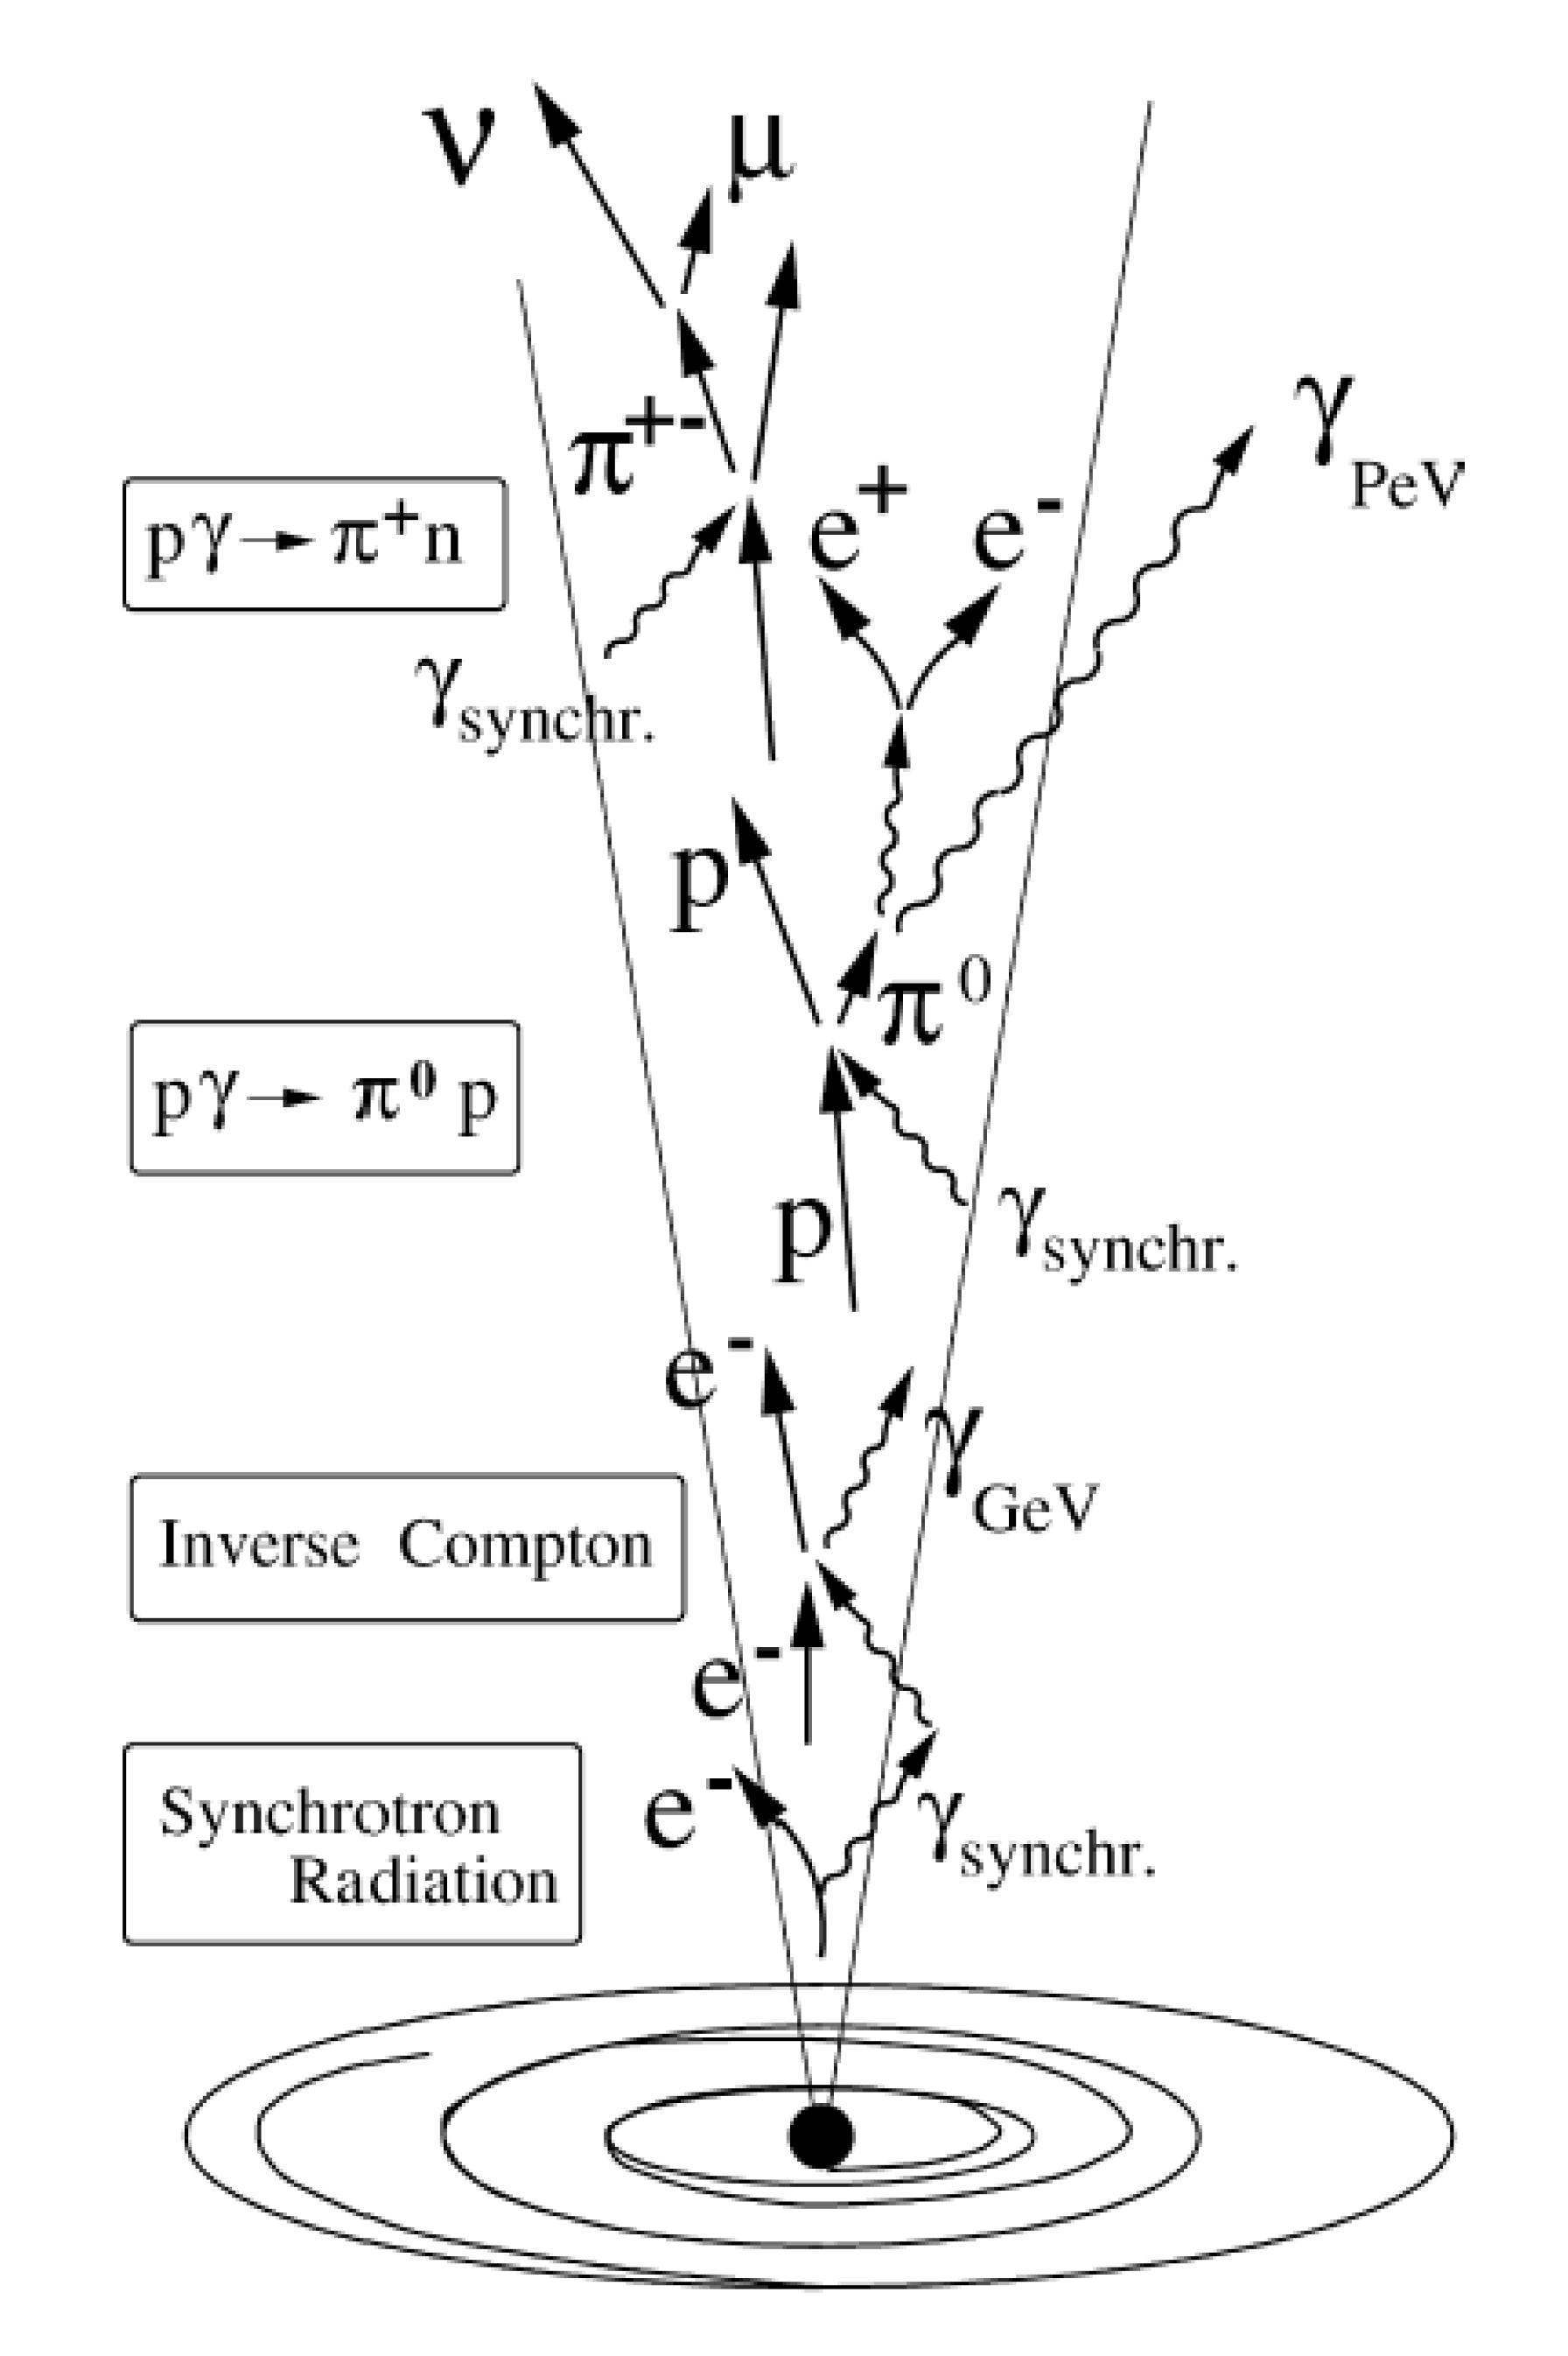
\includegraphics[keepaspectratio,height=12cm]{jet}
\end{center}
%
\colorbox{yellow}{Can this GRB fireball model be probed ?}

\newpage

\begin{center}
{\blue Neutrino production mechanism}\\[5mm]
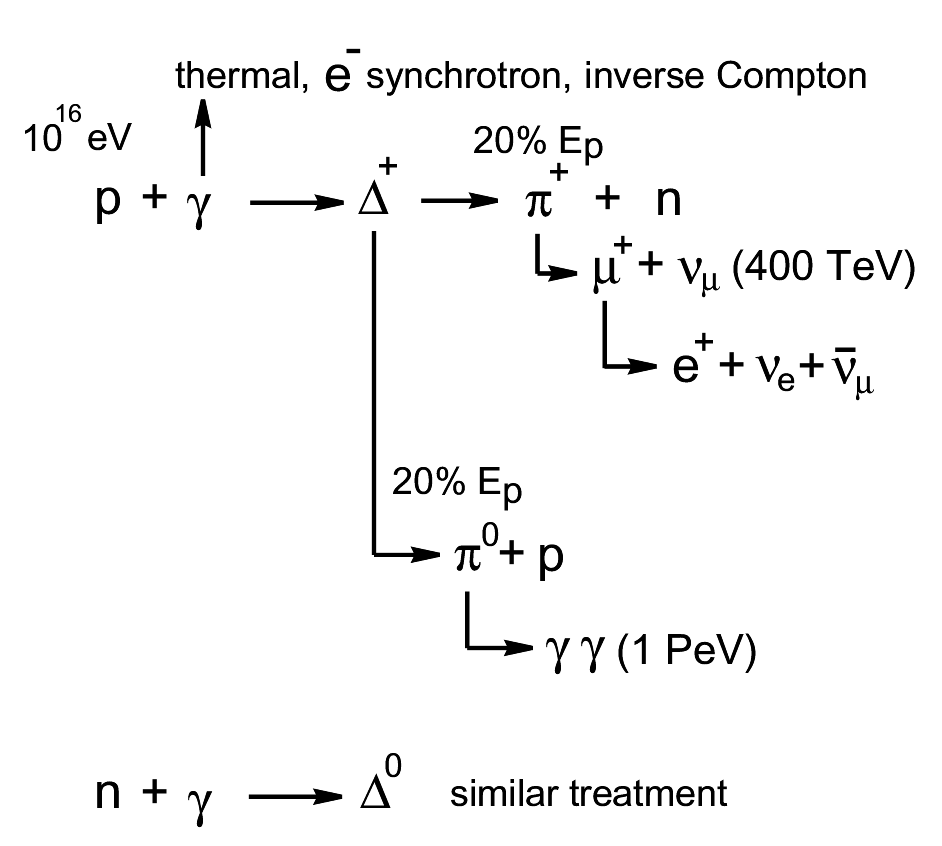
\includegraphics[keepaspectratio,width=12cm]{grb-engine2}
\end{center}
%
$\Delta$ production threshold~: $E_{\gamma} \ge 10$ eV\\
(UV photons)

\Transcb{yellow}{blue}{Observation of high-energy photons}
\vspace*{1cm}
\begin{center}
{\blue Compton Gamma Ray Observatory}\\[5mm]
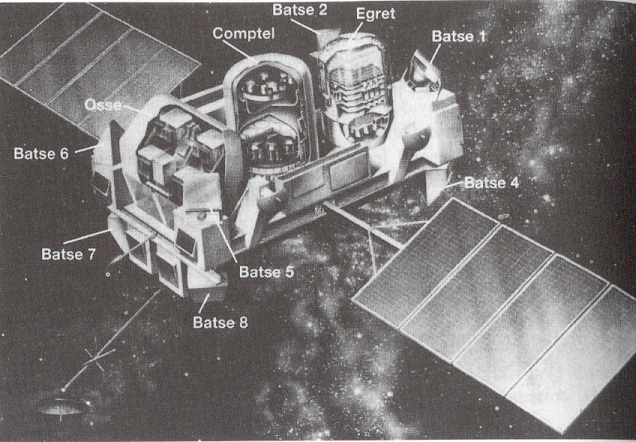
\includegraphics[keepaspectratio,width=12cm]{cgro}
\end{center}

\newpage
\vspace*{2mm}
%
\begin{itemize}
\item COMPTEL (sky maps, spectroscopy)
\item[] Compton Telescope
\item[] Wide field 1-30 MeV
{\blue
\item EGRET (AGN, GRBs, Pulsars)
\item[] Energetic Gamma Ray Exp. Telescope
\item[] Wide field 20 MeV - 30 GeV
}
\item OSSE (X-ray sources, QSO spectra, SNe)
\item[] Oscillating Scintillation Spectrometer Exp.
\item[] Narrow field ($4^{0} \times 11^{0}$) 50 keV - 10 MeV
{\blue
\item BATSE (All sky monitor, GRBs)
\item[] Burst and Transient Source Experiment
\item[] Wide field (8 elements) 20 keV - 30 MeV
}
\end{itemize}

\Tr
\vspace*{0.5cm}
\begin{center}
{\blue The WHIPPLE gamma ray telescope}\\[5mm]
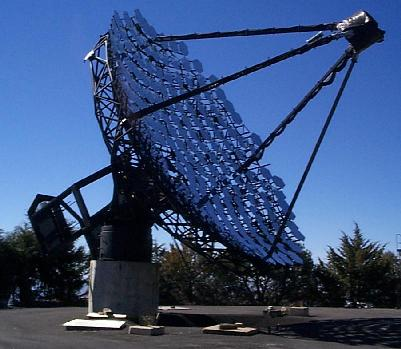
\includegraphics[keepaspectratio,width=12cm]{whipple}
\end{center}

\newpage
\vspace*{3cm}
%
\begin{itemize}
\item Ground based (Arizona, USA)
\item[] Reflective 10 meter diameter dish
\item Cerenkov radiation from air showers
\item[] Field of view : $3^{0}$
\item[] Shower energy 100 GeV - 10 TeV
\end{itemize}

\Tr
\onecolumn
\begin{center}
{\blue Observations of Markarian 421}
\end{center}
%
\begin{itemize}
\item Markarian 421 : AGN at a distance of about 100 Mpc ($z=0.031$).
\item Discovered in 1991 by TeV gamma rays (Nature 160 (1992) 477).
\item Observed by EGRET (1991-1993) and Whipple 1993-1994 : Flare at 14-15 may 1994.
\item[] (ApJ 438 (1995) L59. $\quad$  ApJS 94 (1994) 551.)
\item EGRET ($E_{\gamma}>100$~MeV) : constant flux of $(1.7 \pm 0.3) \cdot 10^{-7}$ photons cm$^{-2}$ s$^{-1}$ 
\item Whipple ($E_{\gamma}>250$~GeV) : average flux of $(2.3 \pm 0.3) \cdot 10^{-11}$ photons cm$^{-2}$ s$^{-1}$ 
\item[] Flux during 1994 flare : $(2.1 \pm 0.3) \cdot 10^{-10}$ photons cm$^{-2}$ s$^{-1}$ 
\end{itemize}

\begin{center}
\colorbox{yellow}{Can the fireball model be probed ?}\\[5mm]
in other words :\\[5mm]
\colorbox{yellow}{Can we indicate hadronic processes in these objects ?}
\end{center}
%
Even more violent transient phenomena are observed ...
\Tr
\twocolumn
\begin{center}
{\blue Batse GRB trigger 109}\\[5mm]
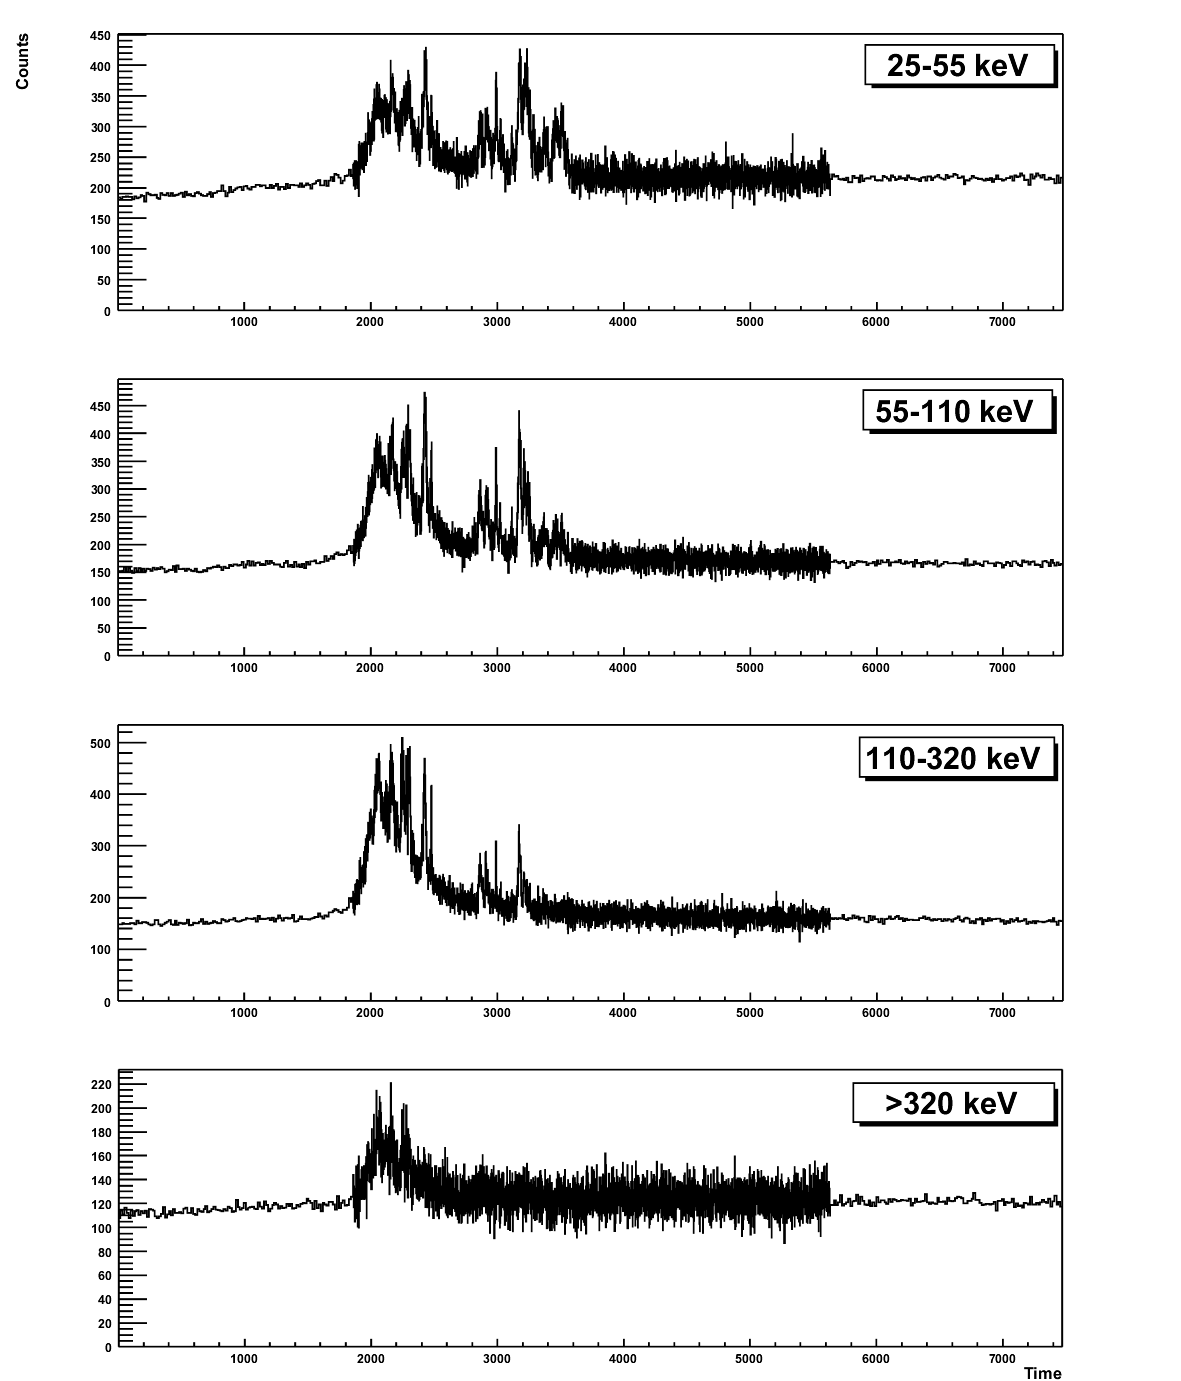
\includegraphics[keepaspectratio,height=14cm]{batse-109}
\end{center}

\newpage

\vspace*{2cm}
%
\begin{itemize}
\item Burst lasts $\sim$2 minutes
\item Rich (energy dependent ?) structure
\begin{itemize}
\item Rather compact source involved
\item Process might consist of several phases
\item[] Various shock waves ?
\end{itemize}
\item[] What are these GRBs ?
\begin{itemize}
\item Common features ?
\item Where are they located ?
\end{itemize}
\end{itemize}

\Tr
\twocolumn[\begin{center}{\blue Burst duration analysis}\end{center}]
%
\vspace*{0.5cm}
%
\begin{center}
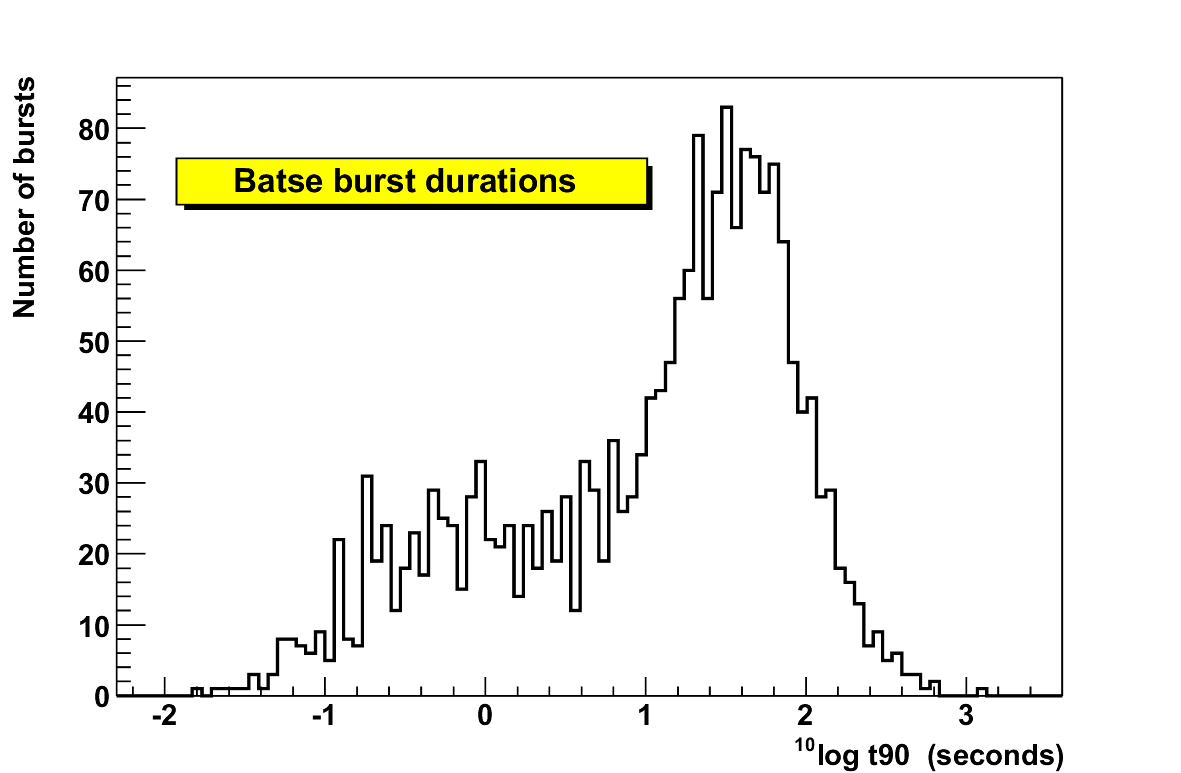
\includegraphics[keepaspectratio,width=13cm]{batse-logt90}
\end{center}

\newpage

\vspace*{1cm}
%
\begin{itemize}
\item t90 $\equiv \Delta t$ from 5\% to 95\% of fluence
\item Two classes : short and long bursts ?
\begin{itemize}
\item Long : dense medium (hypernovae ?)
\item Short : dilute medium (mergers ?)
\end{itemize}
\item[] {\blue Effect of (cosmological) time dilation ?}
\end{itemize}

\Tr
\twocolumn[\begin{center}{\blue Time spectrum analysis}\end{center}]
%
\begin{center}
{\red Possible source of time structure}\\[5mm]
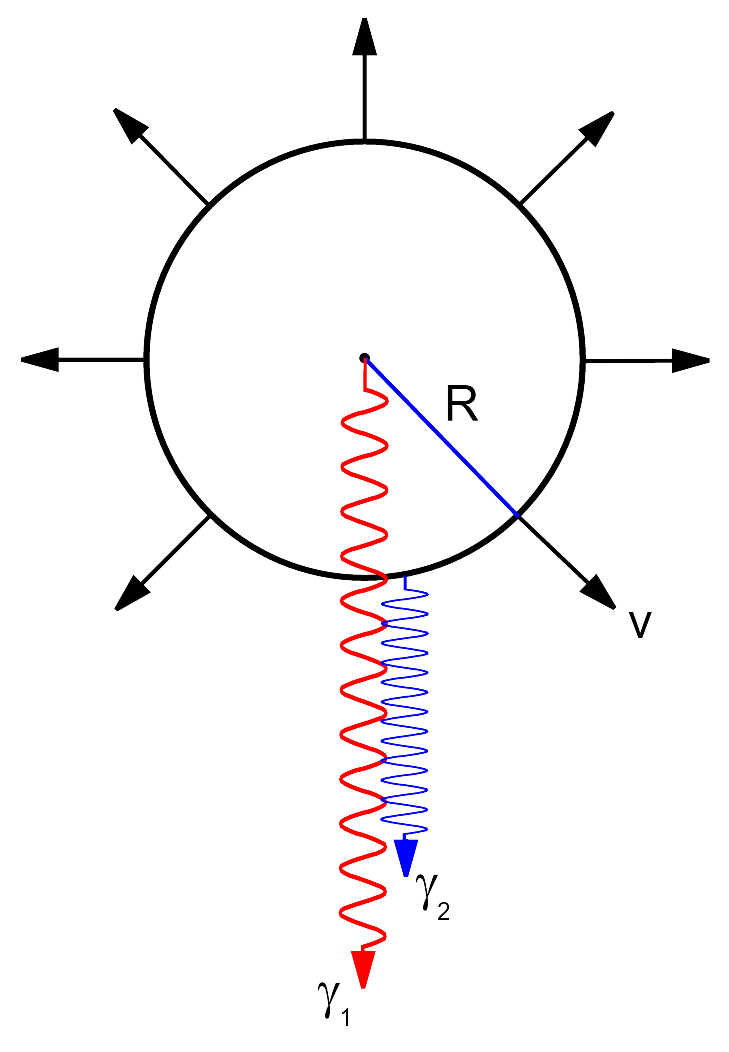
\includegraphics[keepaspectratio,height=10cm]{grb-shell3}
\end{center}
%
\begin{itemize}
\item If distance $r$ can be determined (see later)
\item[] $\rightarrow$ (Cosm.) time dilation correction known
\end{itemize}

\newpage

\begin{itemize}
\item Consider center of GRB as origin at rest
\item[] $\gamma_{1}$ produced at $t_{1}=0$
\item[] $\gamma_{2}$ produced at $t_{2}=t_{1}+R/v$
\item[] At some time $t>t_{2}$ we have
\item[] $r_{1}=ct$ and $r_{2}=R+c(t-R/v)$
\item $\gamma_{1}$ and $\gamma_{2}$ observed at the earth
\item[] $\displaystyle \Delta t=\frac{r_{1}-r_{2}}{c}=\frac{R}{c}\left(\frac{1}{\beta}-1\right)$
\item[] $\displaystyle \rightarrow \Delta t=\frac{R}{v}(1-\beta)
          \approx \frac{R}{v \gamma^{2}} \quad (\gamma \gg 1)$
\item[] {\blue Origin of the various spectral peaks~?}
\item Characteristic size $R$~?
\item[] Would allow determination of $\gamma$ factor
\end{itemize}

\Tr
\begin{center}
{\red Another source of time structure}
\end{center}

\vspace*{0.5cm}

\begin{itemize}
\item[] 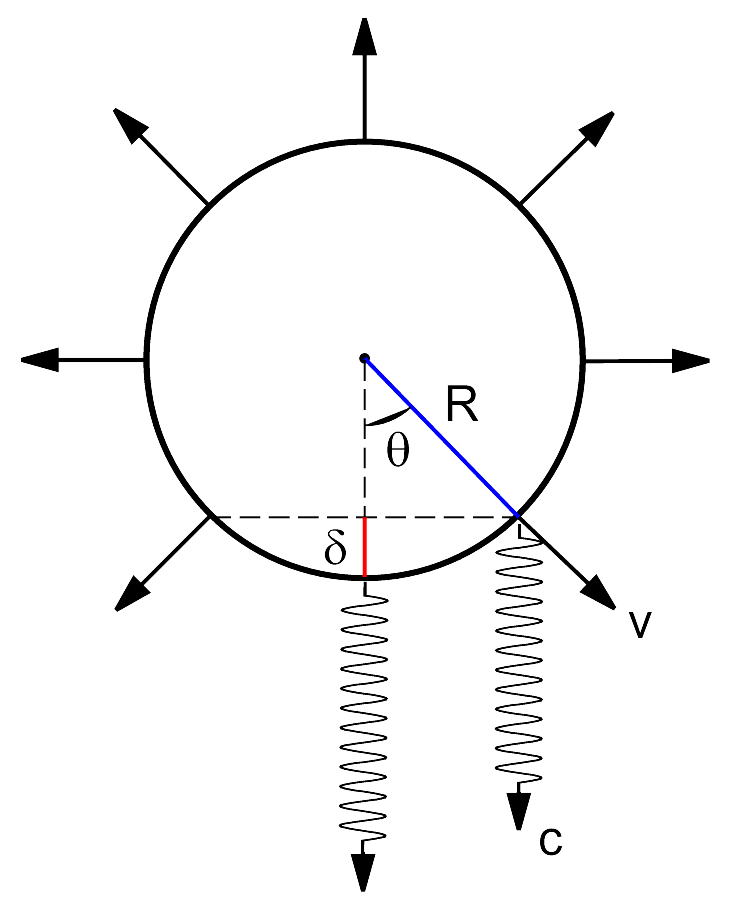
\includegraphics[keepaspectratio,height=7cm]{grb-shell1}
        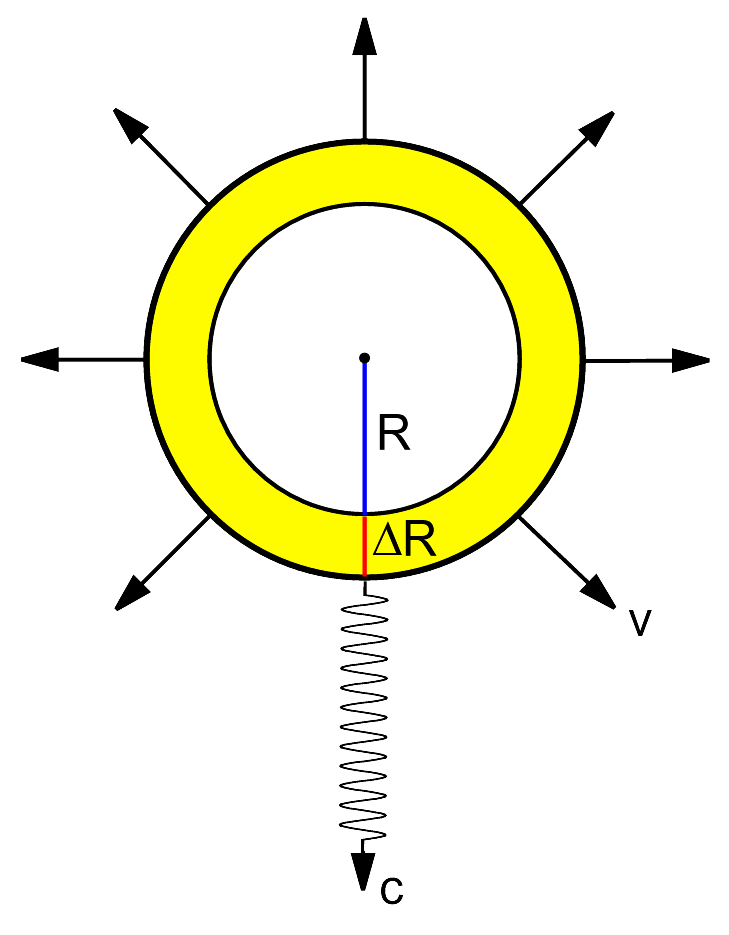
\includegraphics[keepaspectratio,height=7cm]{grb-shell2}
\item Observed duration $\Delta t \rightarrow R$ and $\Delta R$\\[2mm]
      $\displaystyle \Delta t=\frac{\delta}{c}=\frac{R}{c}\left(1-\cos\theta\right)$\\[2mm]
      $\rightarrow R=c\Delta t \quad$ Also : $\Delta R=c\Delta t$
\end{itemize}

\newpage

\vspace*{2.5cm}

\begin{itemize}
\item Quantities in CMS ($\ast$) via inverse Lorentz transformation of observables
\item[] Expanding shell $\rightarrow \gamma$
\item[] Cosmic expansion $\rightarrow \Gamma$
\item So we have ($\gamma \gg \Gamma$)
\item[] $\quad R^{\ast}=\Gamma R \qquad \Delta R^{\ast}=\gamma \Delta R$
\item[] $\quad E^{\ast}=\gamma^{-1} E$
\item {\blue Origin of the width of the peaks~?}
\end{itemize}

\Tr
\twocolumn[\begin{center}{\blue Burst location analysis}\end{center}]
%
\begin{center}
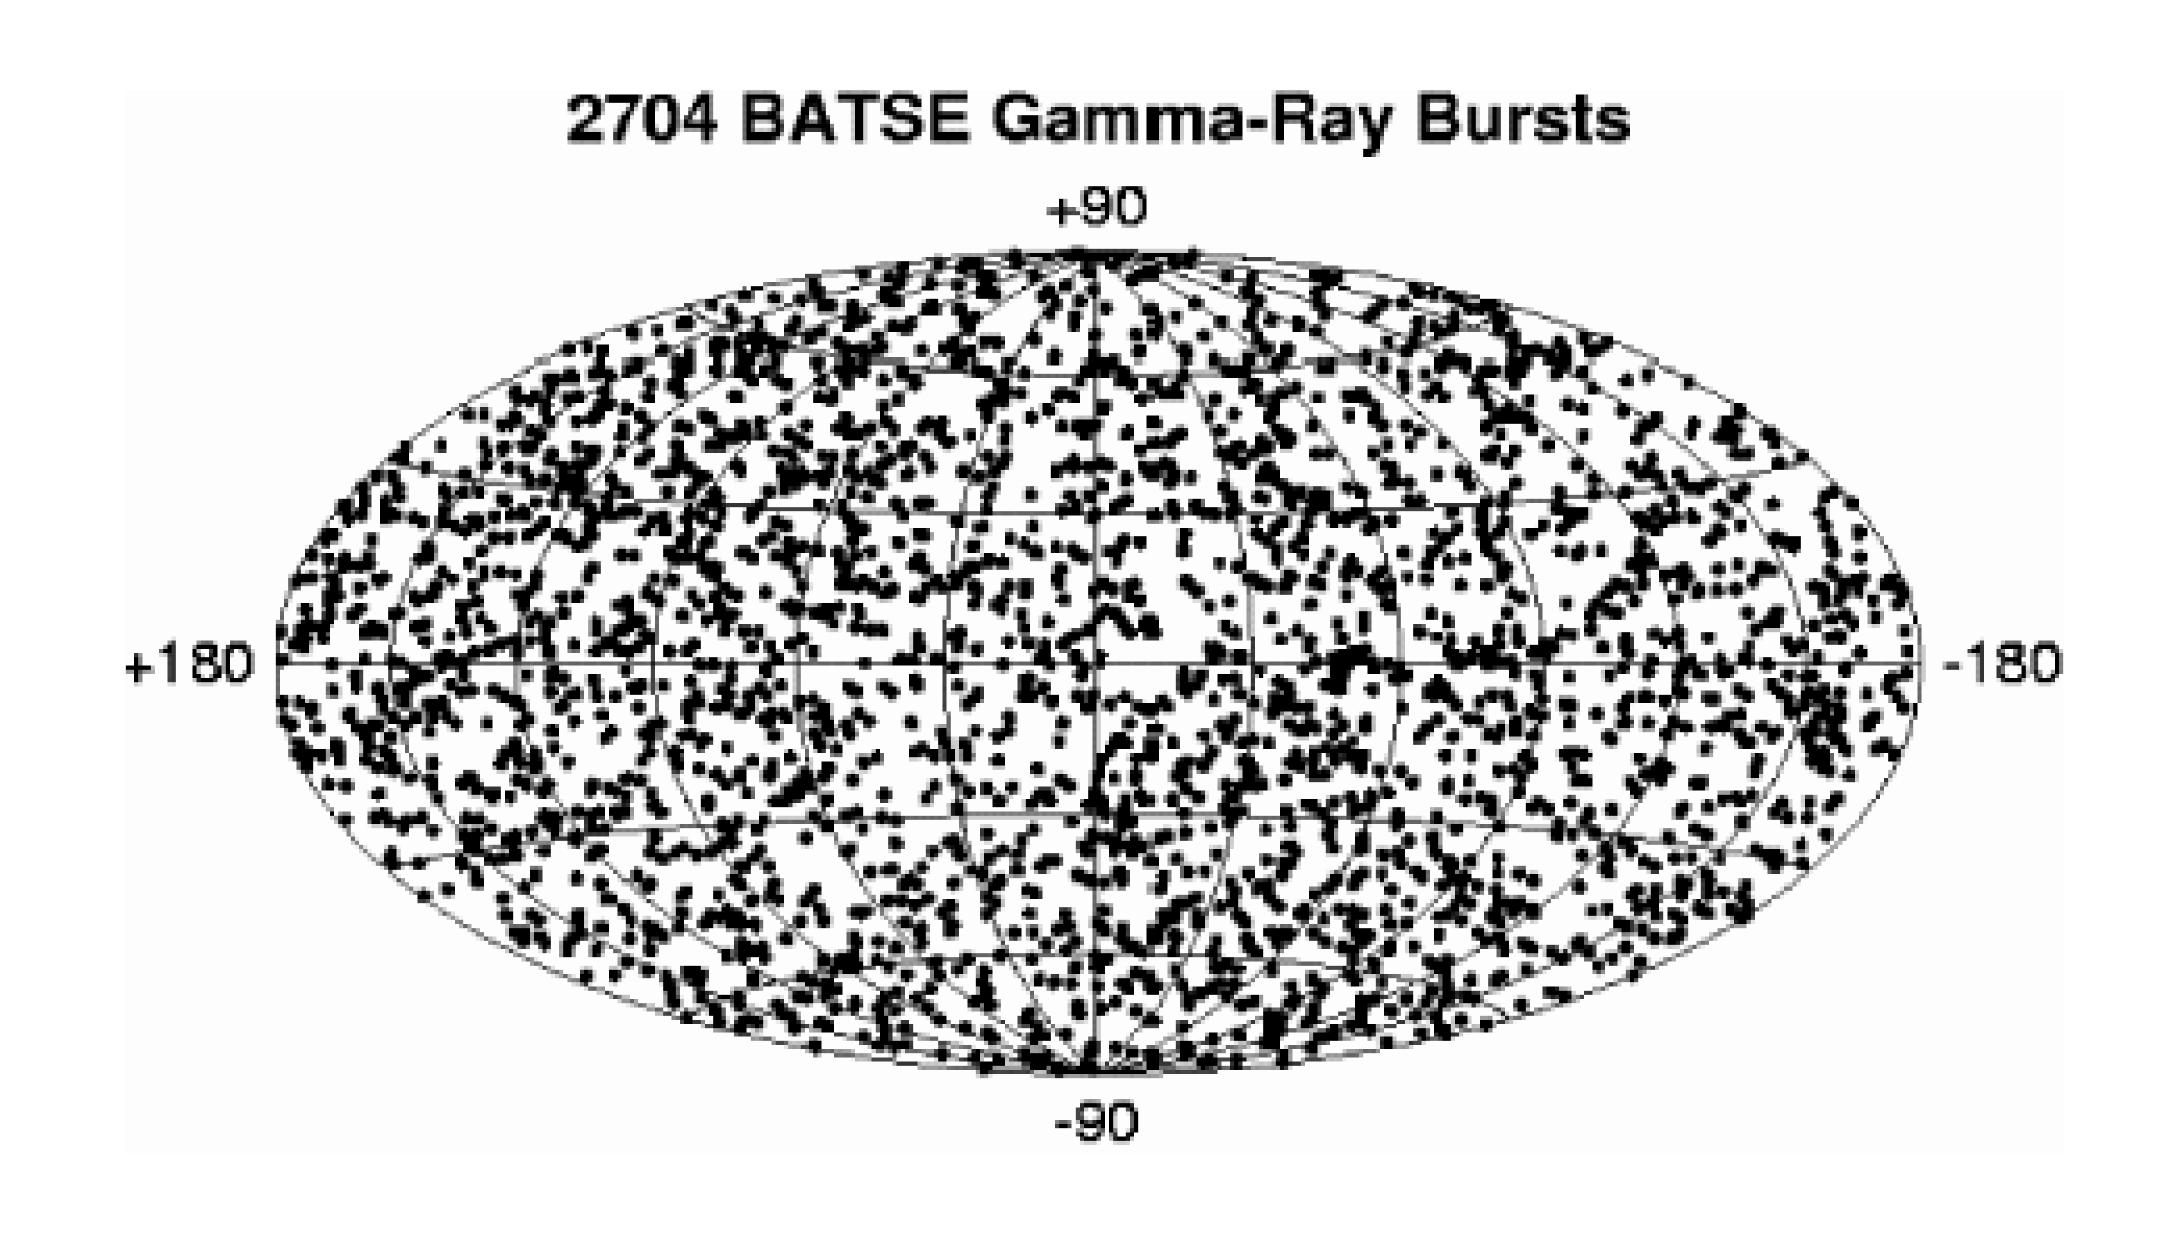
\includegraphics[keepaspectratio,width=13cm]{grbmap}
\end{center}
%
\begin{itemize}
\item No concentration along galactic plane
\item[] $\rightarrow$ Sources of cosmological origin
\item[] Confirmed by afterglow ($z$ values)
\item $(1+z)=\gamma(1+\beta) \quad$ (small $z$)
\item[] $\rightarrow \beta=\frac{(1+z)^{2}-1}{(1+z)^{2}+1}$ and $v=H_{0}r$
\end{itemize}
%
\begin{center}
{\red $z$ and Batse fluence yield total $E$}\\[3mm]
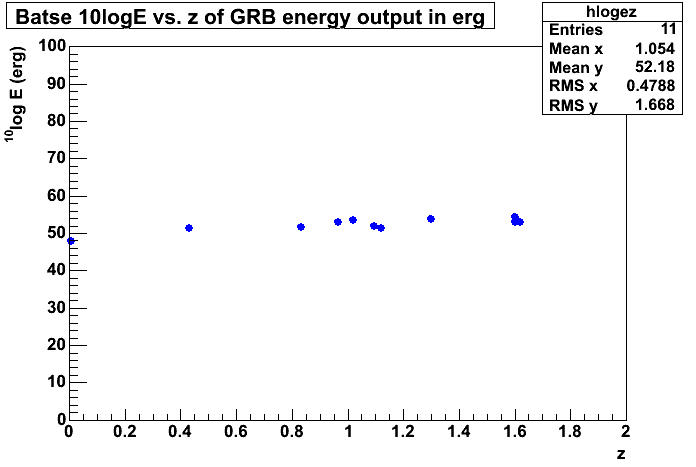
\includegraphics[keepaspectratio,width=13cm]{batse-loge-z}\\
No beaming and $H_{0}=71$ km/s Mpc$^{-1}$
\end{center}
%
\begin{itemize}
\item Characteristic energy output 
\item[] In Batse energy window $E_{0} \sim 10^{52}$ erg
\begin{itemize}
\item Allows to investigate distance distr.
\end{itemize}
\end{itemize}

\Tr
\begin{itemize}
\item Batse observed fluence $S$\\
      and assume $E_{0}$ for all bursts
\item[] $E_{0}=4\pi r^{2} S \rightarrow r=\left(\frac{E_{0}}{4\pi S}\right)^{1/2}$
\item[] \colorbox{yellow}{Batse data provide distance distribution}
\item $S=S_{0}$\\
      $\rightarrow$ specific distance $r_{0}=\left(\frac{E_{0}}{4\pi S_{0}}\right)^{1/2}$
\item[] Obviously $r < r_{0} \rightarrow S > S_{0}$
\item[] Homogeneous burst density $n$ Mpc$^{-1}$ yr$^{-1}$
\begin{itemize}
\item[] $\rightarrow N(>S_{0})=n\frac{4}{3}\pi r_{0}^{3} \propto S_{0}^{-3/2}$
\end{itemize}
\item[] \colorbox{yellow}{Batse data $N(>S_{0})$ vs. $S_{0}$ probe $n$}
\end{itemize}

\begin{itemize}
\item[$\ast$] {\blue Was there a specific GRB epoch~?}
\item[$\ast$] {\blue Match with cosmic-ray flux at the ankle~?}
\item[] Ankle~: $E^{2}\,\frac{\d N}{\d E} \approx 10^{-7}$ GeV cm$^{-2}$ s$^{-1}$
\end{itemize}

\newpage

\vspace*{1cm}

\begin{center}
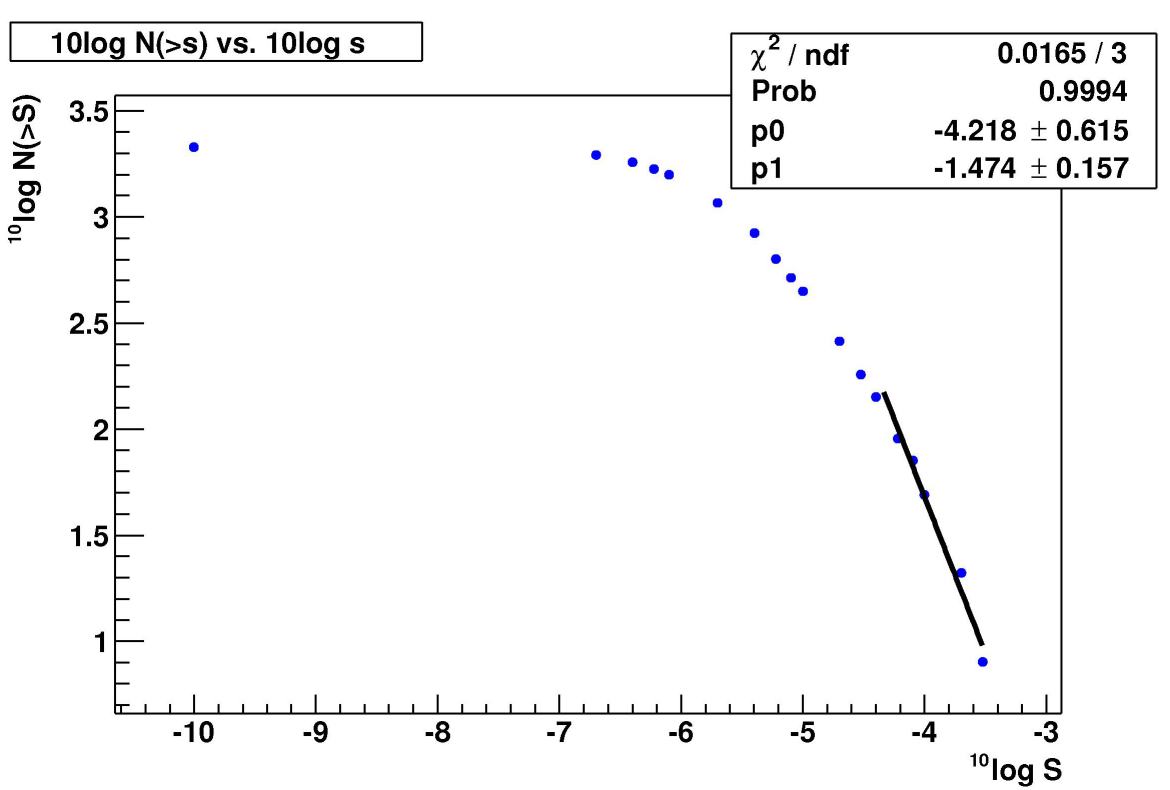
\includegraphics[keepaspectratio,width=13cm]{batse-n-s}
\end{center}
%
\begin{itemize}
{\red
\item Correction for redshift needed
\item Watch out for detector thresholds
}
\end{itemize}

\Tr
\onecolumn

\begin{itemize}
\item Using redshift and physical distance~:
      $\displaystyle S_{obs}=\frac{E_{0}}{4\pi (r_{phys})^{2}(1+z)}$\\[1mm]
\item Flat Friedmann-Lema\^{\i}tre universe and Robertson-Walker metric\\[1mm]
\item[] $\displaystyle r_{phys}(z_{obs})=\frac{c}{H_{0}}
        \int_{z=0}^{z=z_{obs}} \frac{\d z}{\sqrt{\Omega_{M}(1+z)^{3}+\Omega_{\Lambda}}}$\\[1mm]
\item[$\ast$] WMAP \& Planck observations (2013) : $\Omega_{M}=0.315 \pm 0.017 \quad \Omega_{\Lambda}=0.685 \pm 0.017$
\item[] $\rightarrow$ Integral needs to be solved numerically
\item[$\ast$] Simplified model~: $\Omega_{M}=1 \quad \Omega_{\Lambda}=0$
              $\displaystyle \rightarrow r_{phys}=\frac{2c}{H_{0}}\left( 1-\frac{1}{\sqrt{1+z}} \right)$\\[1mm]
\item $N(>S_{0})$ vs. $S_{0}$ analysis with simplified model yields~:
      $n=1.7 \cdot 10^{-10}$ Mpc$^{-3}$ yr$^{-1}$
\end{itemize}

\twocolumn

\Transcb{yellow}{blue}{Link with cosmic rays}
\onecolumn

\begin{itemize}
\item Assume UHECR fluence originates from GRBs~:
      $\displaystyle S_{obs}=\frac{E_{cr}}{4\pi (r_{phys})^{2}(1+z)}$\\[1mm]
\item Spherical shell of thickness $\d r \rightarrow \d N=n \cdot 4\pi r_{phys}^{2} \d r$ GRBs per year
\item CR flux observed on earth originating from this shell~:
      $\displaystyle F_{shell}(r)=S\,dN=\frac{E_{cr}n\,\d r}{1+z}$
\item Total CR flux observed on earth~:
      $\displaystyle F_{cr}=\int_{r=0}^{r_{max}} \frac{E_{cr}n\,\d r}{1+z}$
\item Simplified model for $r_{phys}(z) \rightarrow$
      $\displaystyle F_{cr}=\int_{0}^{\infty} \frac{c E_{cr} n \, \d z}{H_{0}(1+z)^{3/2}}
       =\frac{2cE_{cr}n}{3H_{0}}$
\item Taking $E_{cr}=10^{52}$ erg $\quad n=1.7 \cdot 10^{-10}$ Mpc$^{-3}$ yr$^{-1}$
\item[] $\rightarrow F_{cr} \approx 10^{-8}$ GeV cm$^{-2}$ s$^{-1} \quad$
        (observed $\approx 10^{-7}$ GeV cm$^{-2}$ s$^{-1}$)
\item[] Not a bad result for a simplified model !
\end{itemize}

\begin{center}
\colorbox{yellow}{What sort of particles could these be and where do they come from~?}
\end{center}

\Tr
\onecolumn
\begin{center}
{\blue It's a long and difficult journey}\\[5mm]
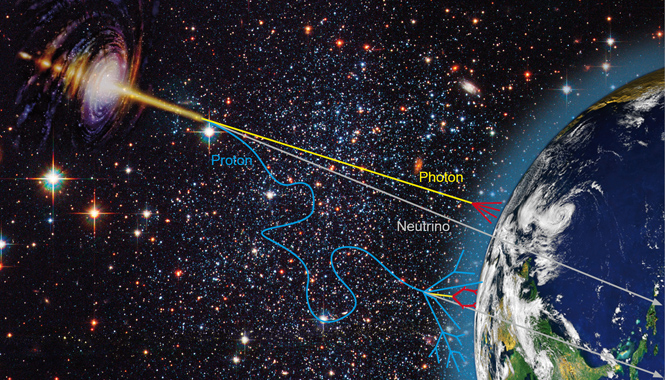
\includegraphics[keepaspectratio,height=13cm]{app}\\[5mm]
\colorbox{yellow}{Only photons and neutrinos point back to the source}
\end{center}

\twocolumn

\Transcb{yellow}{blue}{Hunting for Cosmic Neutrino sources}
\twocolumn
\begin{center}
\colorbox{yellow}{Neutrino production mechanism}\\
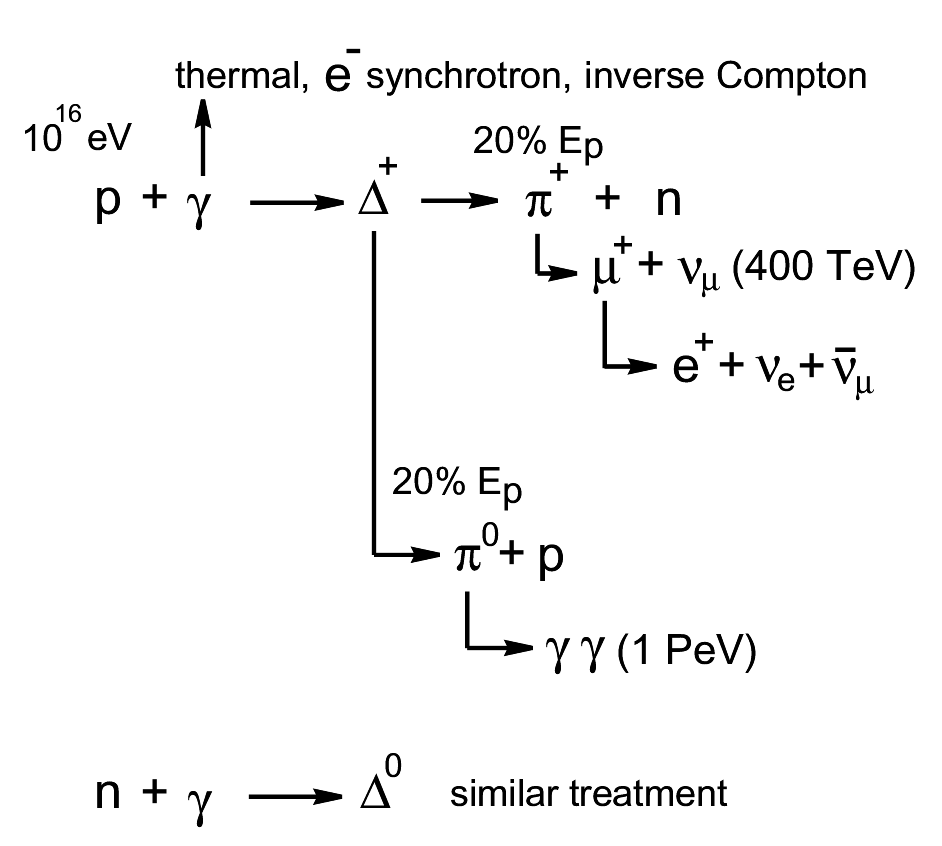
\includegraphics[keepaspectratio,width=13cm]{grb-engine2}
\end{center}
%
\begin{itemize}
\item $\Delta$ prod. threshold~: $E_{\gamma} \ge 10$ eV\\
      (UV photons)
\end{itemize}

\newpage
%
\begin{itemize}
\item Waxmann-Bahcall model
\item[] High-E $p$ diffuse out of the shocks
\item[] Observed CR $\rightarrow$ lower limit on $p$ flux 
\item[] {\blue Fraction of $p$ used for $\nu$ production ?}
\item Magn. confinement (Rachen, Ahlers)
\item[] Protons trapped, neutrons escape
\item[] CR observations provide the $n$ flux 
\item[] {\blue Direct relation CR $\leftrightarrow \nu$ flux}
\item Non-Cosmic Ray (Guetta, H\"{u}mmer)
\item[] Fixed fraction of $E_{\gamma}$ outflow as $p$
\item[] Protons not necessarily escape
\item[] {\blue Normalisation of proton fraction ?}
\item[] {\blue Fraction of $p$ used for $\nu$ production ?}
\item[$\ast$] \colorbox{yellow}{Let's search for high-E $\nu$ sources}
\end{itemize}

\Tr
\onecolumn
\begin{center}
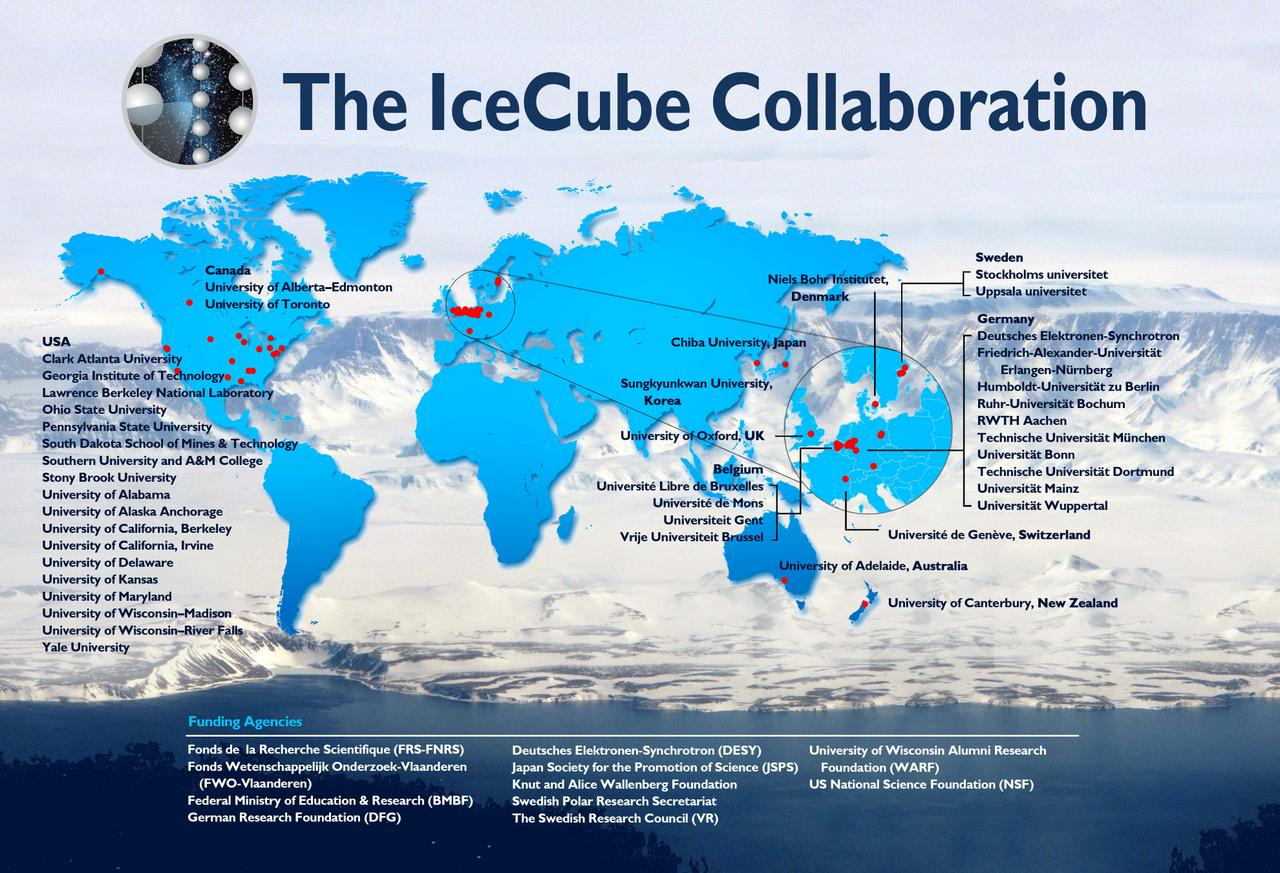
\includegraphics[keepaspectratio,height=15cm]{icecube-collab}
\end{center}

\Tr
\onecolumn
\begin{center}
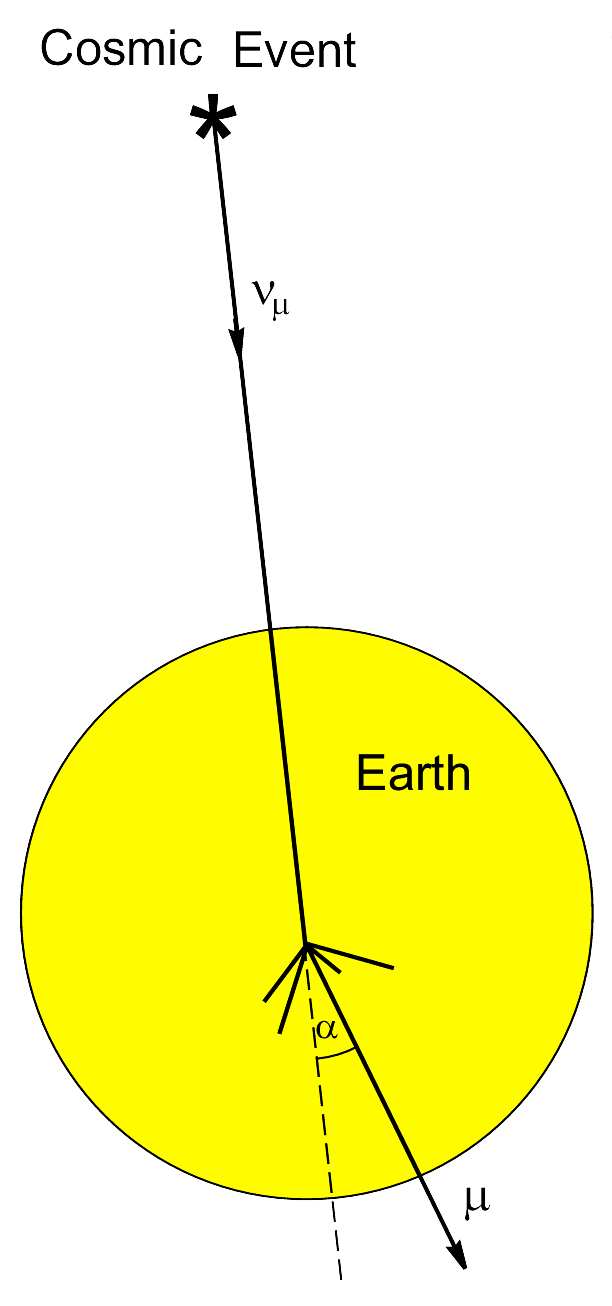
\includegraphics[keepaspectratio,height=14cm]{earth-shield} $\quad$
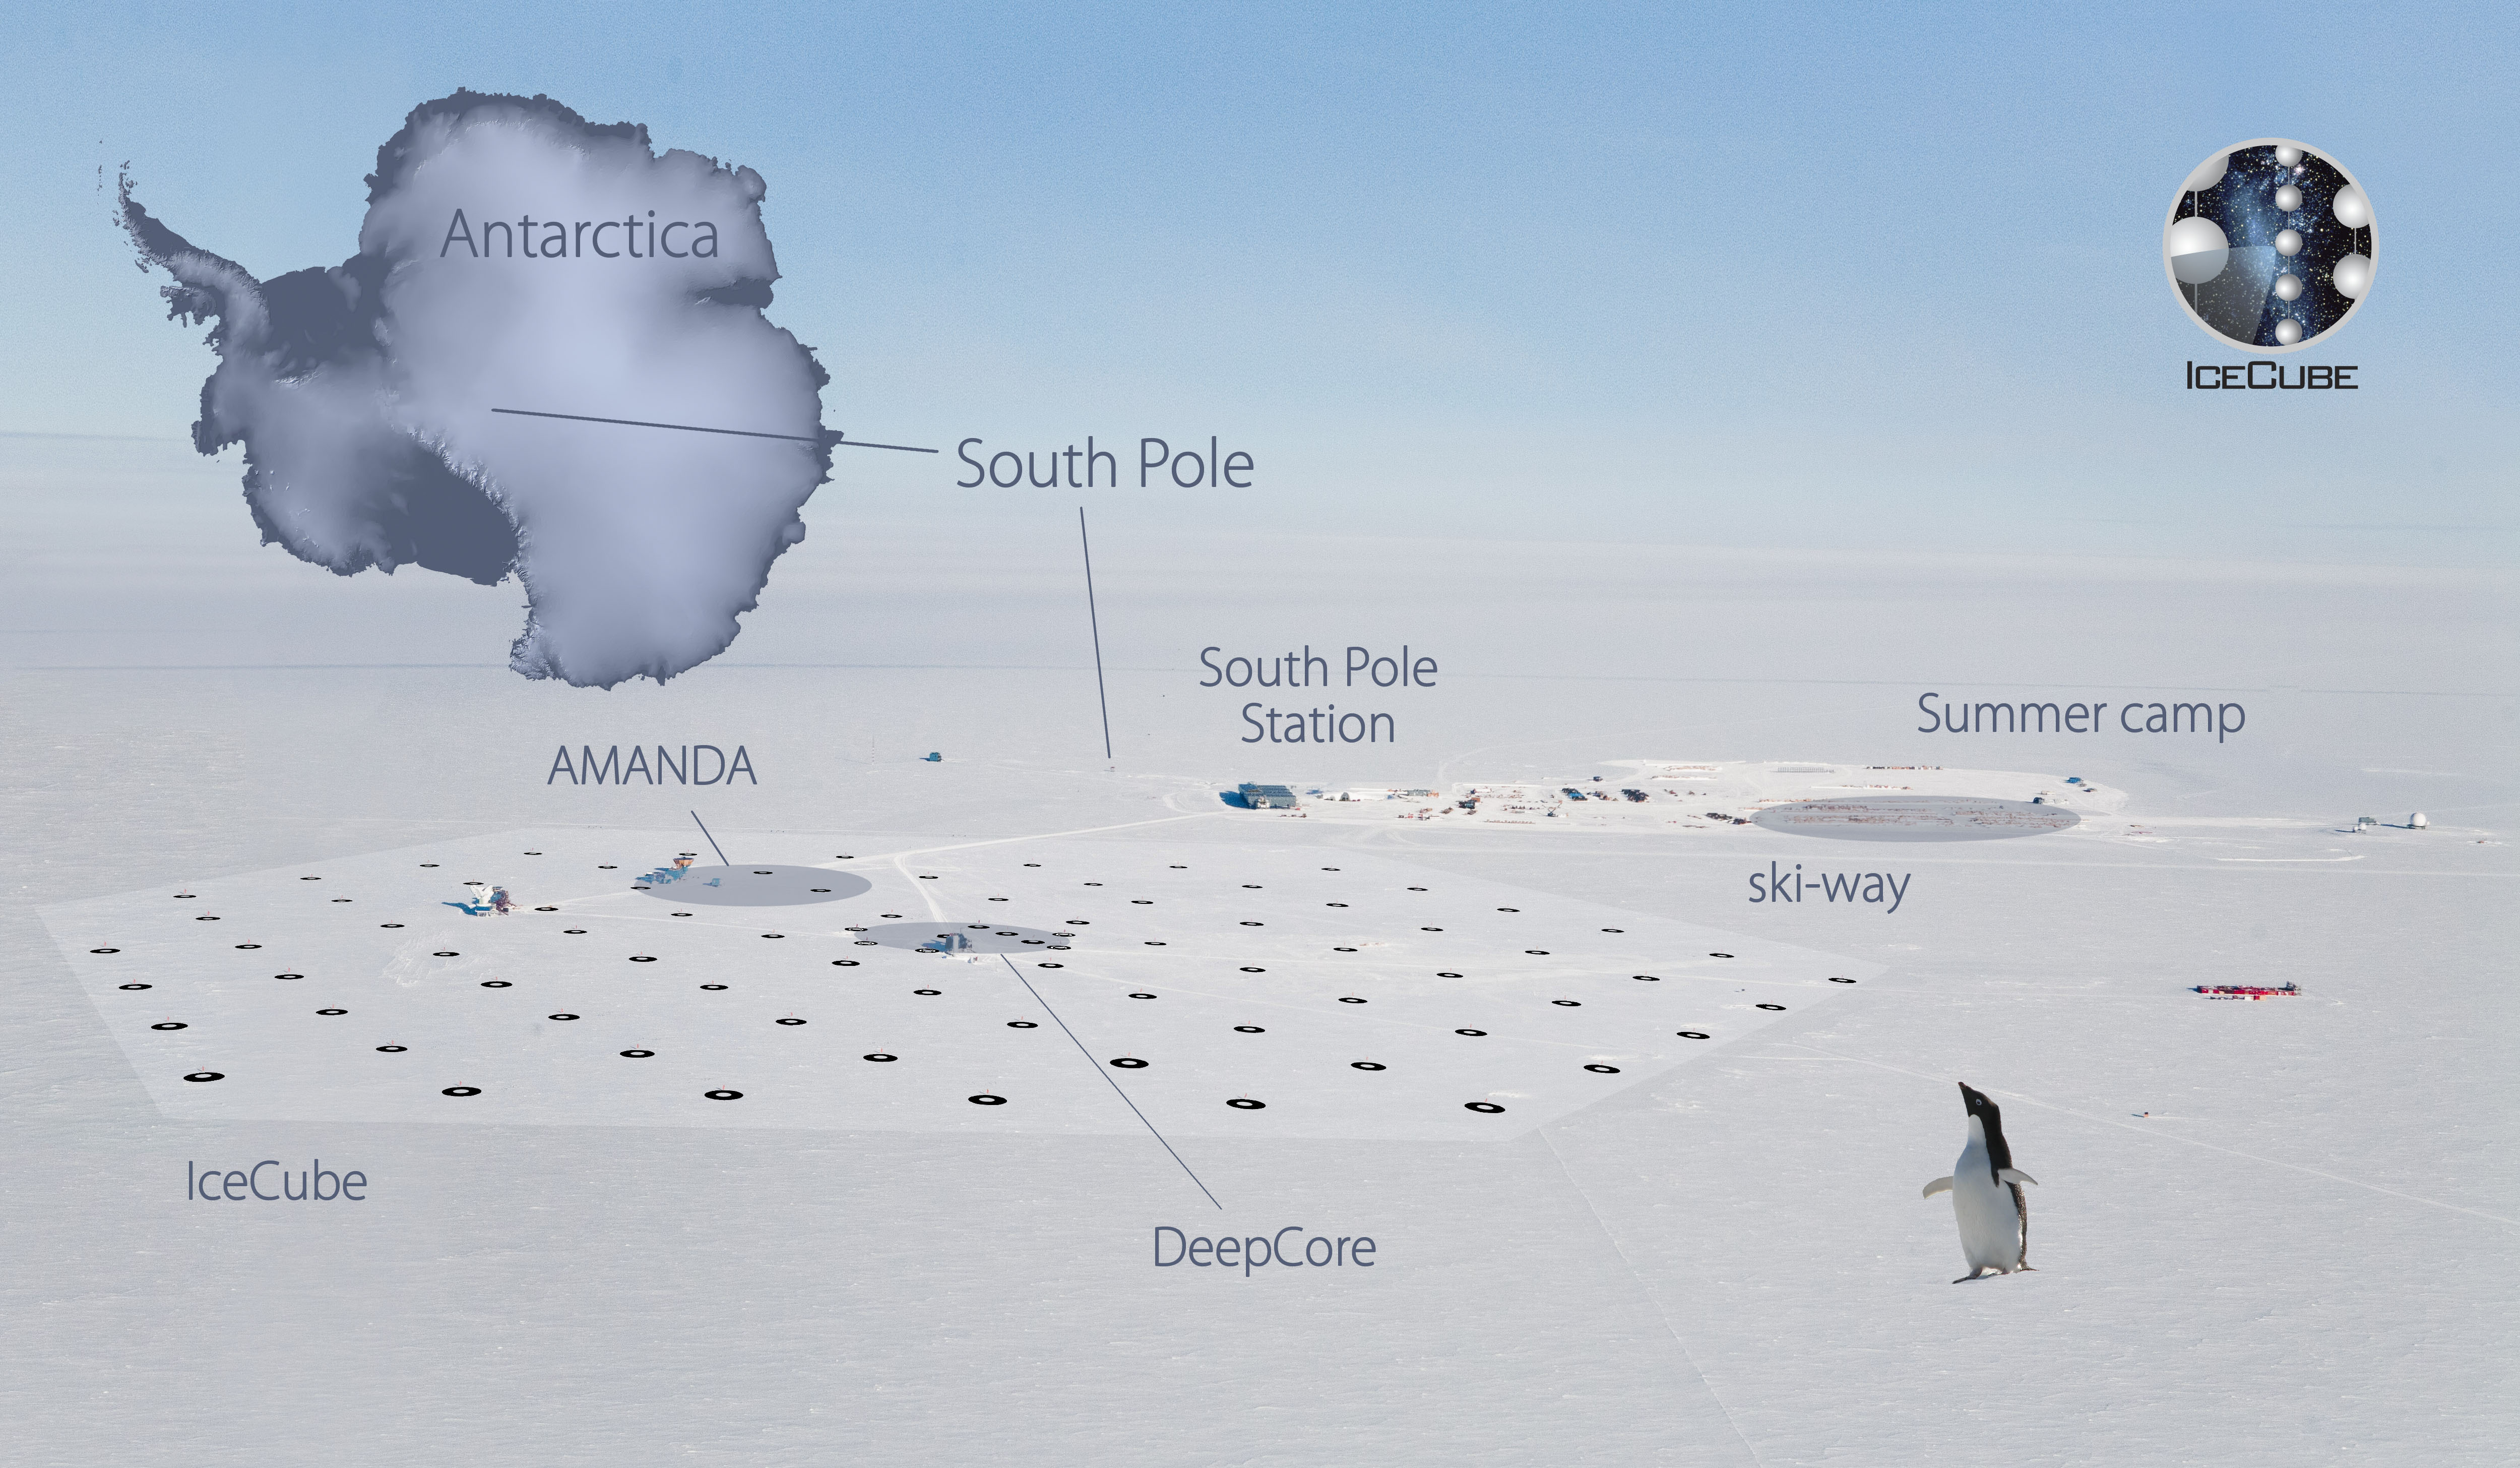
\includegraphics[keepaspectratio,width=18cm]{pole-view}
\end{center}

\Tr
\onecolumn
\begin{center}
{\blue The IceCube neutrino observatory}\\[3mm] 
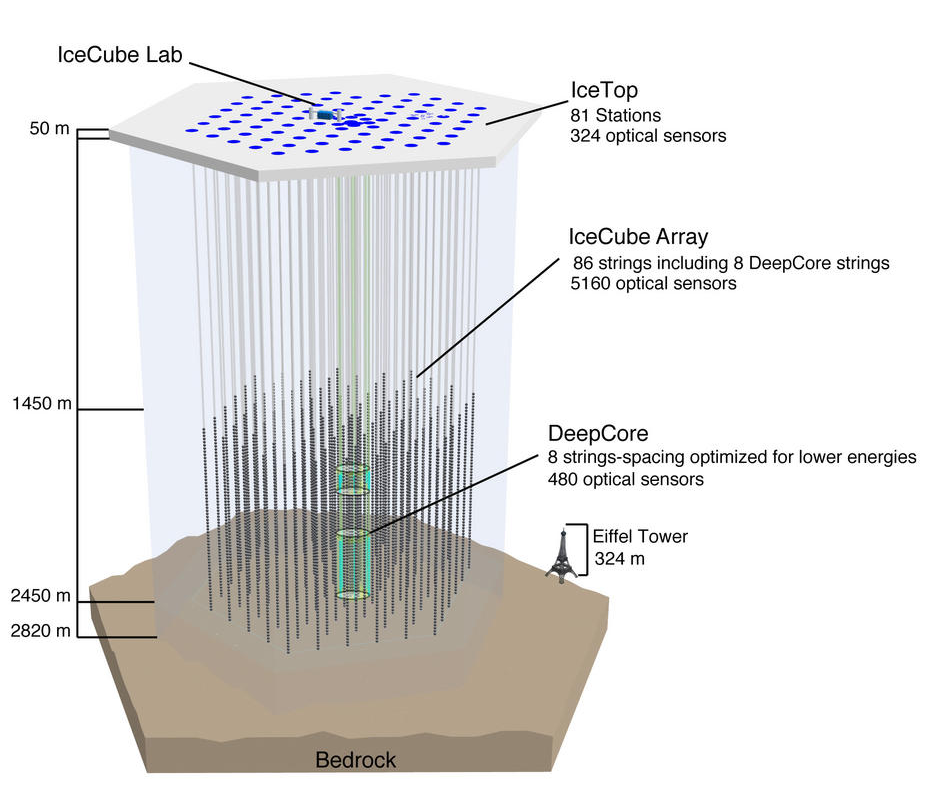
\includegraphics[keepaspectratio,height=14cm]{ic86-dc}
\end{center}

\Tr
\onecolumn
\begin{center}
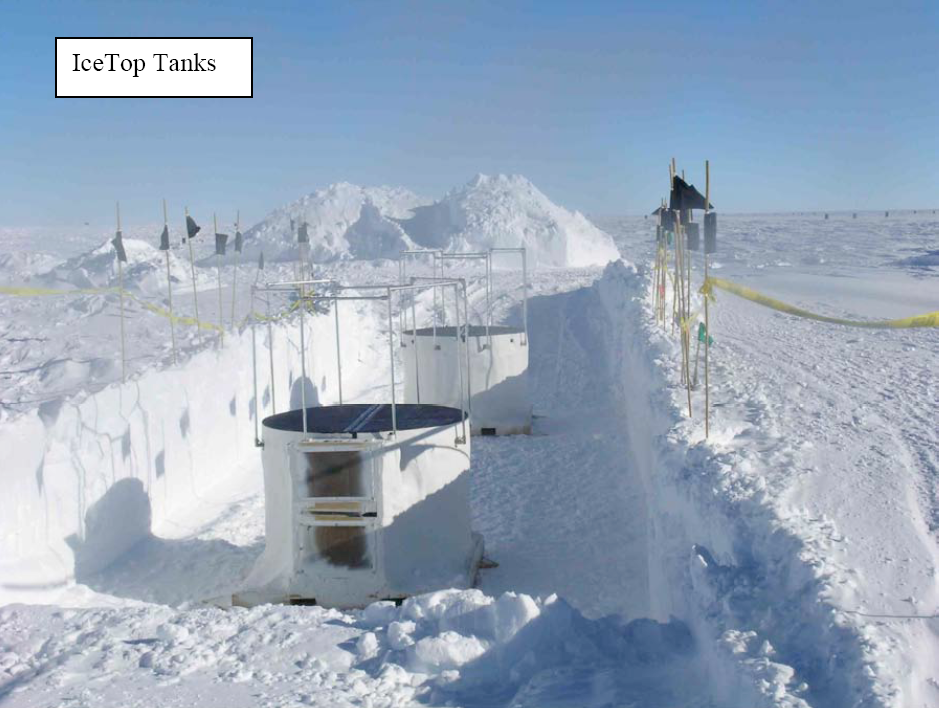
\includegraphics[keepaspectratio,height=14.5cm]{icetop-snow}
\end{center}

\Tr
\onecolumn
\begin{center}
{\blue The IceTop detection principle}\\[5mm] 
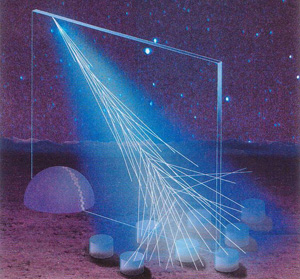
\includegraphics[keepaspectratio,height=14cm]{cr-shower}
\end{center}

\Tr
\onecolumn
\begin{center}
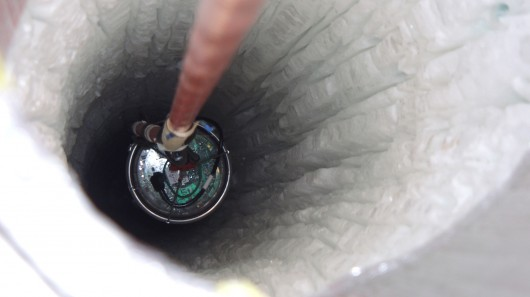
\includegraphics[keepaspectratio,height=14cm]{hole2}
\end{center}

\Tr
\twocolumn[\begin{center}{\blue The InIce detection principle}\end{center}]
\begin{center}
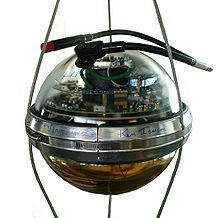
\includegraphics[keepaspectratio,height=6cm]{dom}\\[3mm]
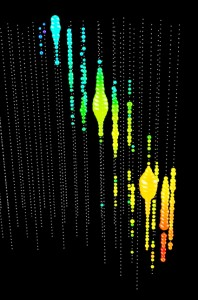
\includegraphics[keepaspectratio,height=7cm]{event}
\end{center}
%
\newpage
%
\begin{center}
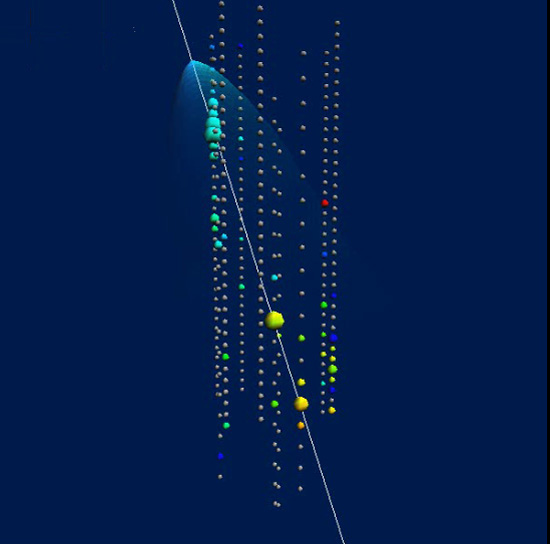
\includegraphics[keepaspectratio,width=13.5cm]{cone}
\end{center}

\Tr
\onecolumn
\begin{center}
{\red Muons from atmospheric interactions}\\[1cm]
{\blue The shadow of the Moon}\\[5mm]
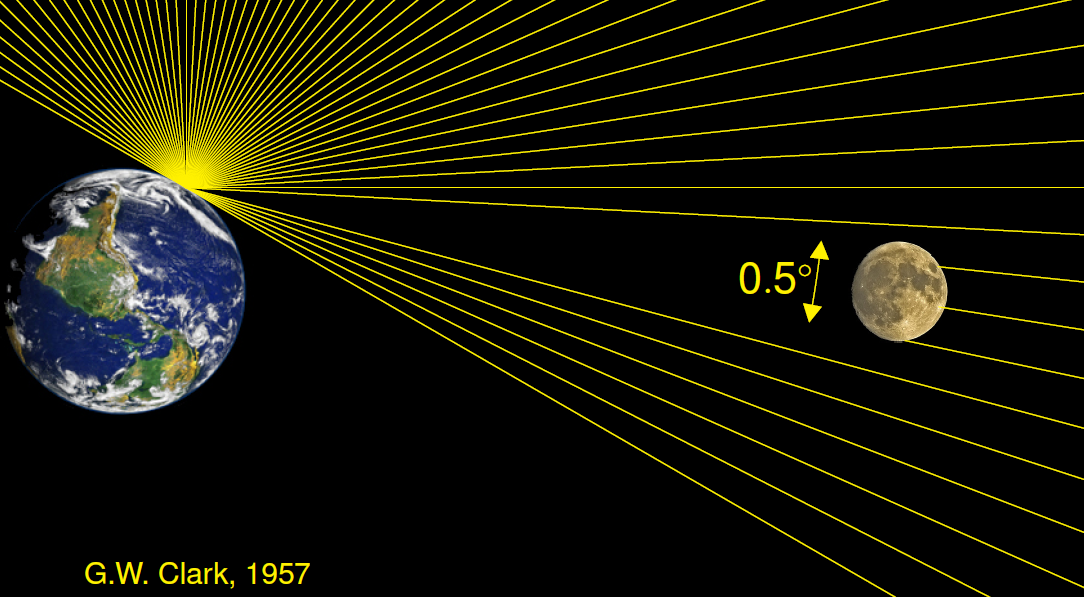
\includegraphics[keepaspectratio,height=8cm]{moon-shadow1}
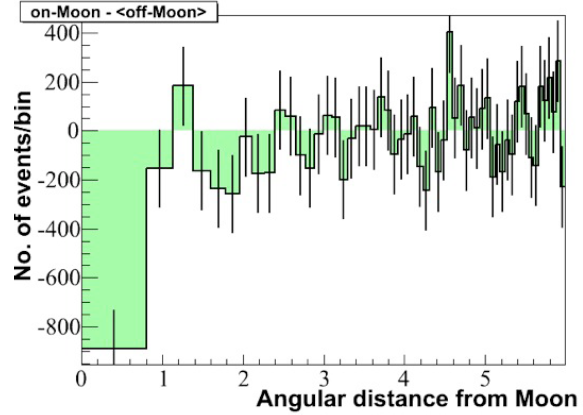
\includegraphics[keepaspectratio,height=8cm]{moon-shadow2}\\[1cm]
{\blue Angular resolution : $\sim 0.8^{\circ}$}
\end{center}

\Tr
\begin{center}
{\red Muons from atmospheric interactions}\\[1cm]
{\blue Cosmic ray anisotropy}\\[5mm]
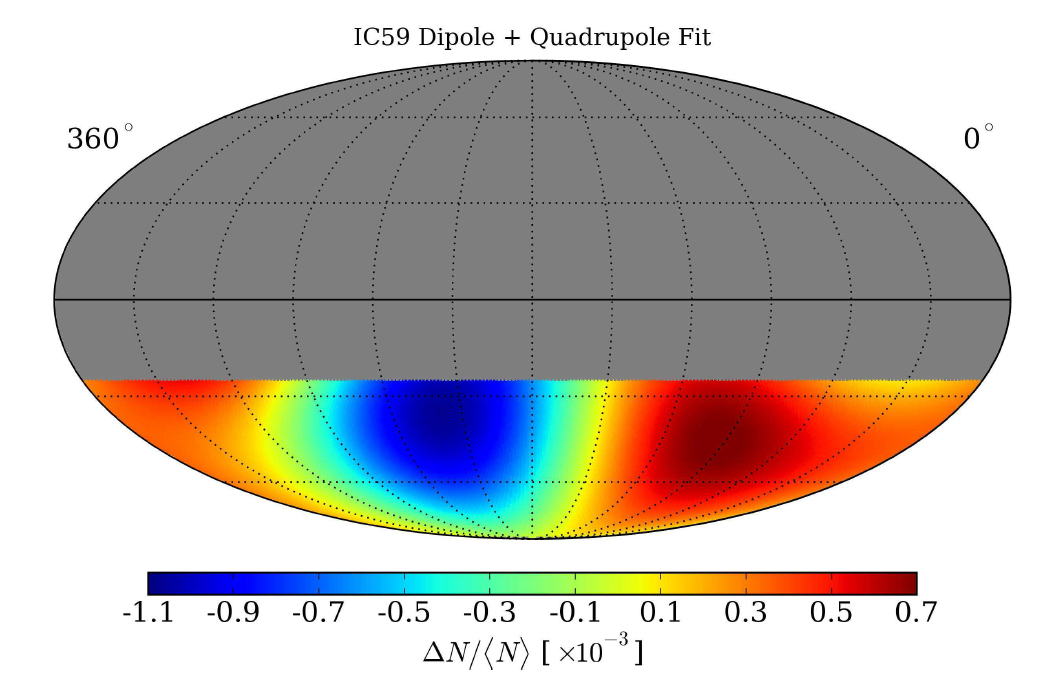
\includegraphics[keepaspectratio,height=12cm]{cr-anisotropy}
\end{center}

\Tr
\onecolumn
\begin{center}
{\blue IceCube neutrino equatorial skymap (ApJ 779 (2013) 132)}\\
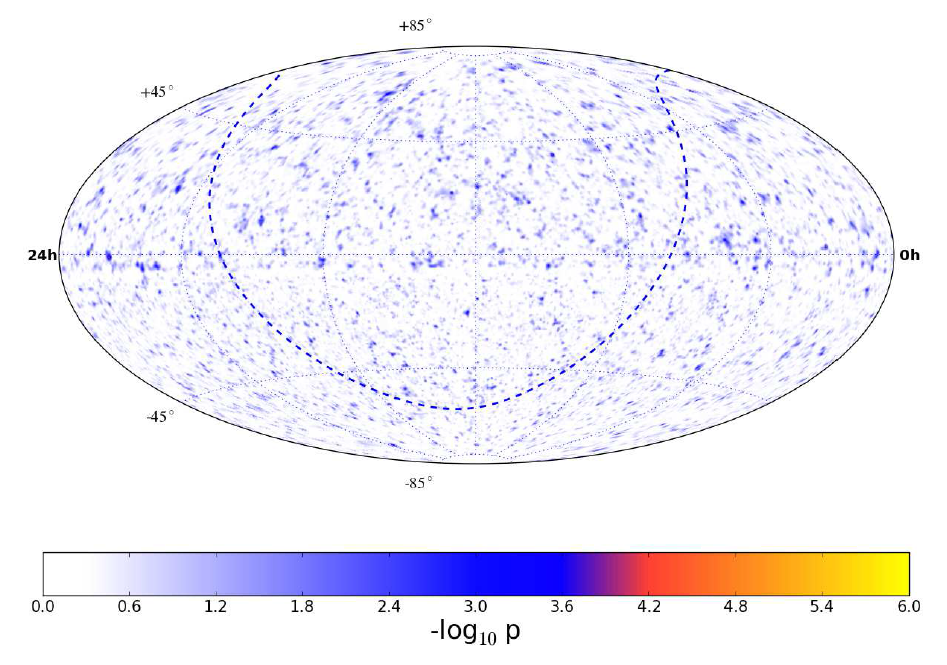
\includegraphics[keepaspectratio,height=12.5cm]{ic79+59+40-skymap}
\end{center}
Most significant excess : $\alpha =$ 2h~17m~0s $\quad \delta = 2.75^{\circ} \quad \text{P-value} = 1.96 \cdot 10^{-5}$\\
Randomised $\alpha$ data sets $\rightarrow$ post-trial : P-value=0.57

\Transcb{yellow}{blue}{Transient cosmic sources}
\twocolumn
\begin{center}
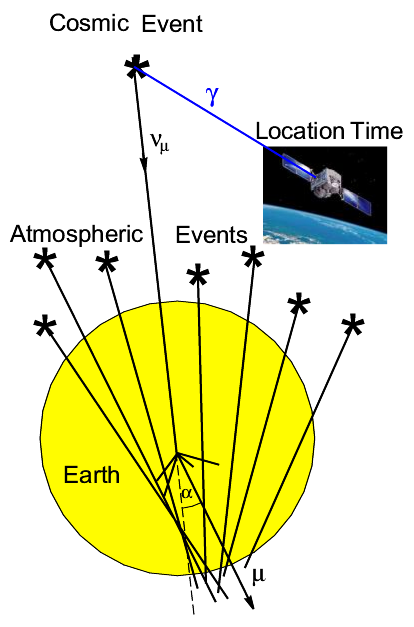
\includegraphics[keepaspectratio,height=15cm]{atm-bkg}
\end{center}

\newpage

\begin{itemize}
\item No signal $\rightarrow$ Give flux upper limit
\item Link observations and flux via Effective area
\item[] $ A_{eff} \equiv$ obs. event rate~/~incoming flux
\item[] $\rightarrow$ Flux limit = max. event rate~/~$A_{eff}$
\end{itemize}
%
\begin{center}
{\blue $\nu_{\mu}+\bar{\nu}_{\mu}$ Effective area (solid angle averaged)}\\
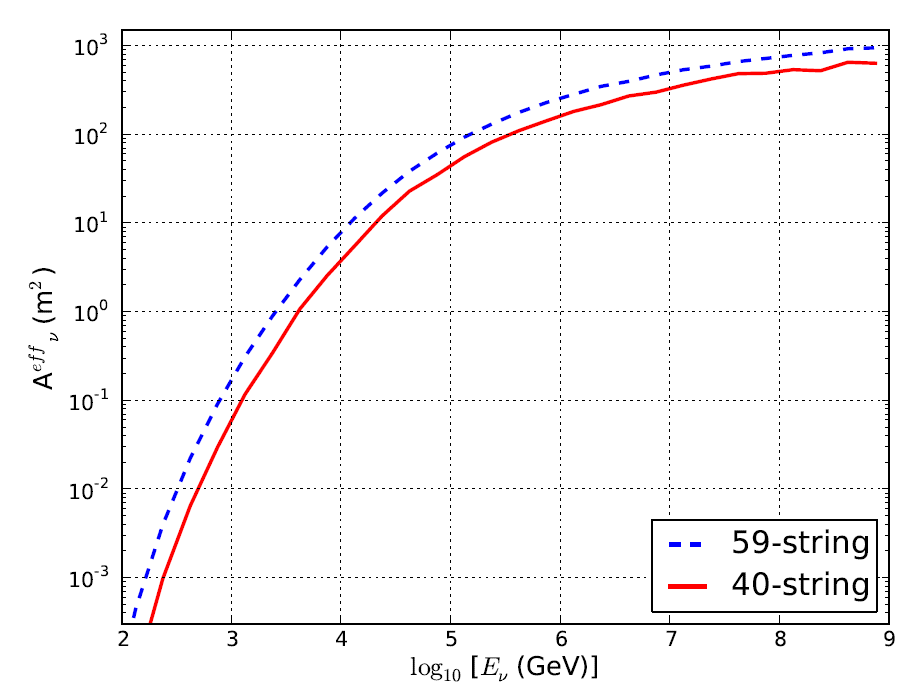
\includegraphics[keepaspectratio,height=9.5cm]{ic59+40-eff-area}
\end{center}

\Tr
\twocolumn
\begin{center}
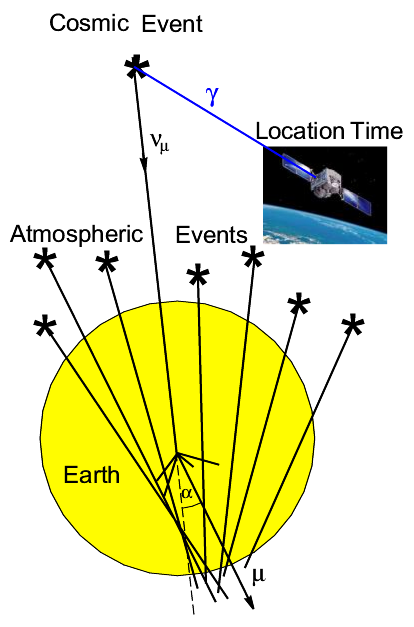
\includegraphics[keepaspectratio,height=15cm]{atm-bkg}
\end{center}

\newpage

\begin{center}
{\red IceCube GRB prompt $\nu$ flux limit}\\
{\large [ApJ Let. 805 (2015) L5]}\\
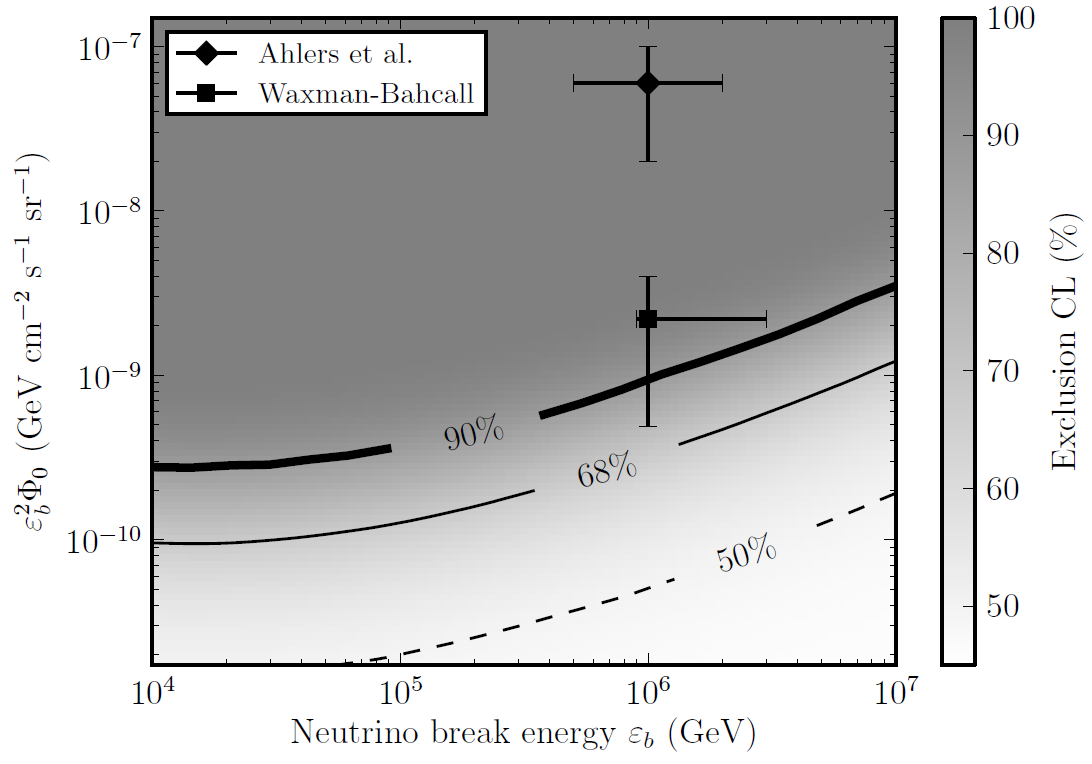
\includegraphics[keepaspectratio,width=13cm]{ic-grb-limit-prompt}
\end{center}
\begin{itemize}
\item[] GRBs not the (only) UHECR sources
\item[] {\blue Or :} $\nu$ prod. lower than expected
\item[] {\blue Or :} $\nu$ prod. outside prompt phase
\end{itemize}

\Transcb{yellow}{blue}{Search for a diffuse cosmic $\nu$ flux}
\twocolumn
\vspace*{5mm}
%
\begin{itemize}
\item Many point sources : diffuse $\nu$ flux
\item[] Expected flux $\sim E^{-2}$
\item[] (Fermi shock acceleration)
\item[] Observed in TeV photons
\item CR primaries : flux $\sim E^{-2.7}$
\item[] $\rightarrow$ Calculate atm. $\nu$ $E$-spectrum
\item IceCube observed atm. $\nu$ spectrum
\item[] Validate calculated spectrum
\item[$\ast$] {\blue PDF for atm. $\nu$ $E$-spectrum}
\item Energy determination is essential
\item[] \colorbox{yellow}{Require contained events}
\end{itemize}

\newpage 
%
%\vspace*{5mm}
\begin{center}
{\blue The atmospheric neutrino spectrum}\\
(ICRC2013)\\
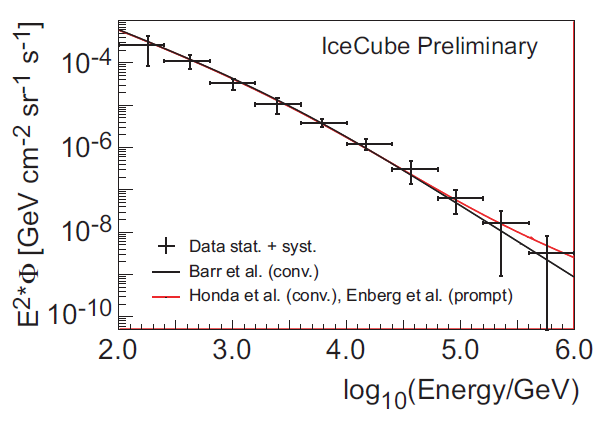
\includegraphics[keepaspectratio,width=13cm]{atm-nu}
\end{center}
%
\begin{itemize}
\item Very high E : Nearly atm. bkg free
\item[] 0.1 atm. $\nu$ per year at 1 PeV
\item[] \colorbox{yellow}{EHE events might prove cosmic $\nu$}
\end{itemize}

\Tr
\begin{center}
{\blue Tue 09-aug-2011 07:23:18 UTC}\\
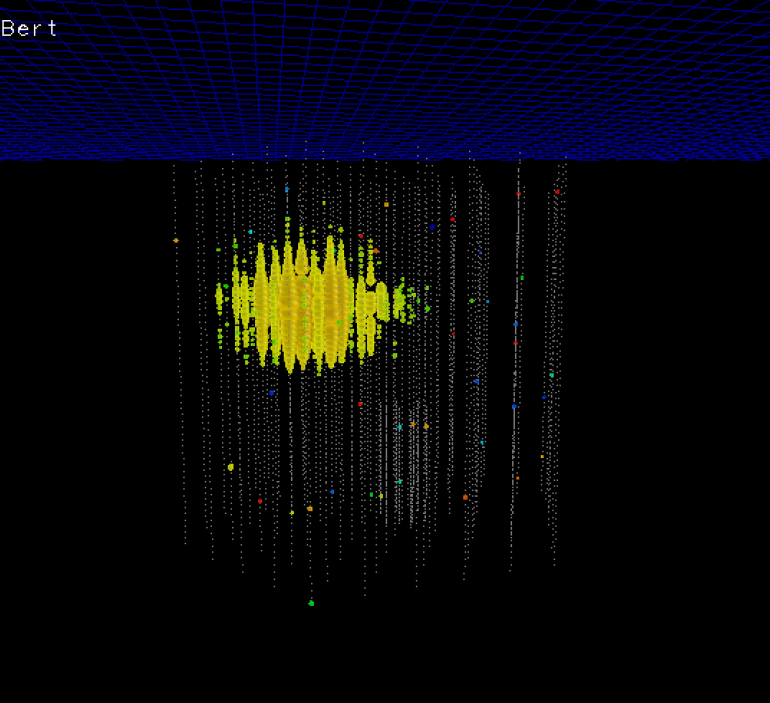
\includegraphics[keepaspectratio,width=13cm]{bert}\\
$1.04 \pm 0.14$ PeV
\end{center}
{\blue Atmospheric $\nu$ background ?}

\newpage

\begin{center}
{\blue Tue 03-jan-2012 03:34:01 UTC}\\
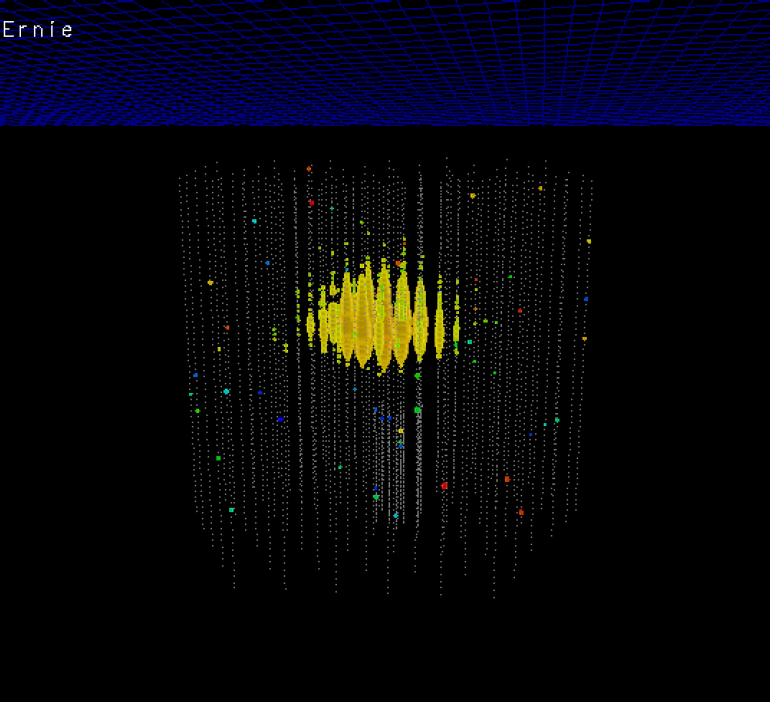
\includegraphics[keepaspectratio,width=13cm]{ernie}\\
$1.14 \pm 0.14$ PeV
\end{center}
{\blue P-value : $2.9 \cdot 10^{-3} \quad (2.8 \sigma)$}

\Tr
\onecolumn
\begin{center}
{\blue Try to get more "Muppets in the basket"}
\end{center}
%
\begin{itemize}
\item Perform a High-Energy Starting Event analysis (may 2010$-$may 2013)
\item[] Use event start veto criteria $\rightarrow$ remove atm. bkg $\mu$ and $\nu$ (showers)
\item[] Guarantees (contained) $\nu$ events and allows lower $E$ cut $\rightarrow 4\pi$
\end{itemize}
%
\begin{center}
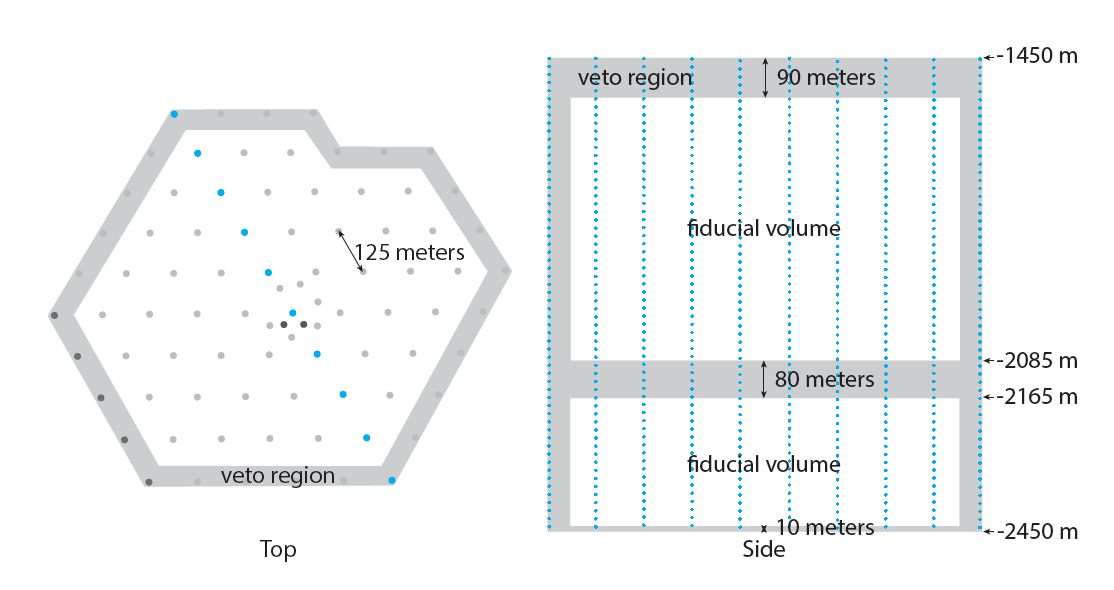
\includegraphics[keepaspectratio,height=10cm]{veto}
\end{center}

\Tr
\twocolumn[\begin{center}{\blue 35 additional events were found}\end{center}]
%
\begin{center}
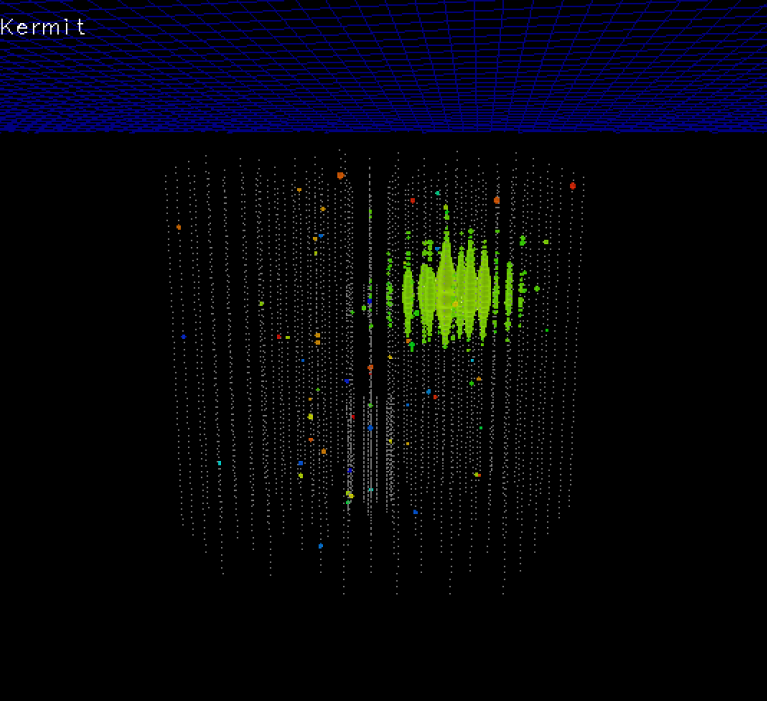
\includegraphics[keepaspectratio,width=13cm]{kermit}
\end{center}

\newpage

\begin{center}
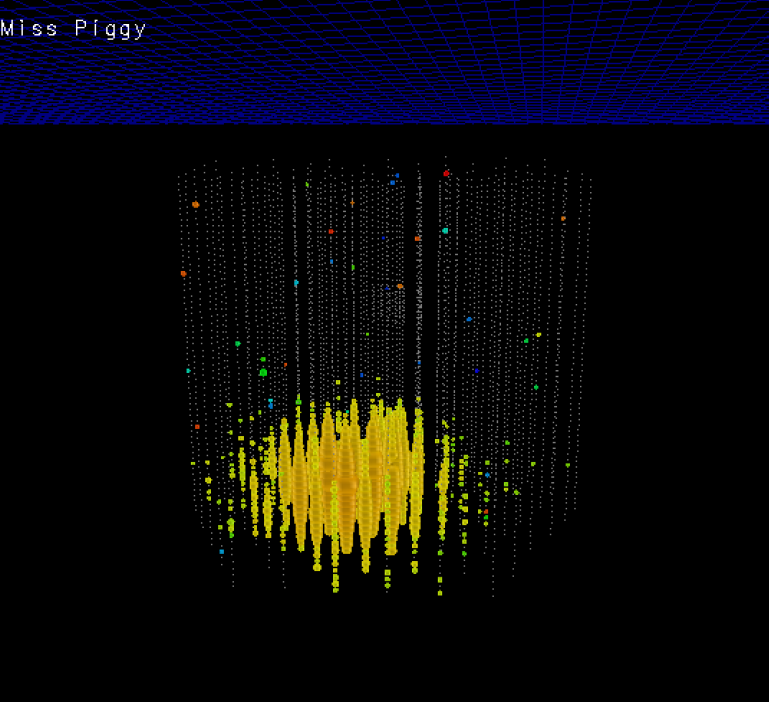
\includegraphics[keepaspectratio,width=13cm]{miss-piggy}
\end{center}

\Tr
\twocolumn[\begin{center}{\blue Also some $\mu$ track signatures}\end{center}]
%
\begin{center}
\includegraphics[keepaspectratio,width=13cm]{dr-strangepork}
\end{center}

\newpage

\begin{center}
\includegraphics[keepaspectratio,width=13cm]{gonzo-the-great}
\end{center}

\Tr
\twocolumn[\begin{center}{\blue Our current champion}\end{center}]
%
\begin{center}
\includegraphics[keepaspectratio,width=13cm]{big-bird}\\
$2.00 \pm 0.25$ PeV
\end{center}

\newpage

\begin{center}
\includegraphics[keepaspectratio,height=12cm]{big-bird-photo}\\
Big Bird
\end{center}

\Tr
\onecolumn
\begin{center}
{\blue Energy distribution of the 37 events}
\end{center}
\includegraphics[keepaspectratio,width=13.5cm]{hese-e}
\includegraphics[keepaspectratio,width=13.5cm]{hese-decl-vs-e}
\begin{center}
\colorbox{yellow}{Evidence for cosmic high-energy neutrinos}
\end{center}

\Tr
\onecolumn
\begin{center}
\includegraphics[keepaspectratio,height=15cm]{breakthrough}\\
\end{center}

\Tr
\onecolumn
\begin{center}
{\blue Cosmic origin confirmed at lower energies}\\[5mm]
{\red IceCube Preliminary}\\
\includegraphics[keepaspectratio,width=25cm]{mese}\\[1cm]
\colorbox{yellow}{IceCube has raised the curtain for Neutrino Astronomy}
\end{center}

\Tr
\onecolumn
\begin{center}
{\blue Source directions of the 37 events}\\
\includegraphics[keepaspectratio,width=20cm]{hese-skymap-gal}\\
\colorbox{yellow}{No evidence for point source(s)}
\end{center}

\Tr
\twocolumn
%
\begin{center}
{\blue The IceCube observed CR anisotropy}\\
(ApJ 740 (2011) 16)\\
\includegraphics[keepaspectratio,width=13cm]{cr-anisotropy}\\[5mm]
\end{center}

\newpage

\begin{center}
{\blue The skymap of our 37 events}\\[1.2cm]
\includegraphics[keepaspectratio,width=13cm]{hese-skymap-equ}\\[5mm]
Investigating correlations might become interesting
\end{center}

\Transcb{yellow}{blue}{The Neutrino-Gamma connection}
\onecolumn
\begin{center}
\includegraphics[keepaspectratio,height=12cm]{Fermi-IC-CR}\\
{\large [Lars Mohrmann, PhD 2015, Humboldt University Berlin]}
\end{center}
%
{\blue
Common astrophysical sources ?\\
$N+\gamma \rightarrow \Delta \rightarrow \pi+{\red N \text{~(CR)}}
 \qquad \pi^{0} \rightarrow {\red \gamma\gamma \text{~(Fermi)}} \qquad \pi^{\pm} \rightarrow {\red \nu,\bar{\nu} \text{~(IceCube)}}$
}

\Tr
\onecolumn
\begin{center}
{\blue Follow up for transients on neutrino alerts}
\includegraphics[keepaspectratio,height=14cm]{IC160427A}\\
{\large [Credit M. Kowalski SuGAR2018]}
\end{center}

\Tr
\onecolumn
\begin{center}
\includegraphics[keepaspectratio,height=14cm]{HESE35}\\
{\large [Credit M. Ahlers SuGAR2018]}
\end{center}

\Tr
\onecolumn
\vspace*{6cm}
\begin{center}
{\red \shabox{\Huge Multi-messenger studies look promising !}}
\end{center}

\Tr
{\blue IceCube: Track with $E_{dep} \sim 24$ TeV observed at 22-sep-2017 20:54:30.43 UTC}\\
$\rightarrow$ EHE alert (IC170922A) issued ($\sim 4$ per year) 
\begin{center}
\includegraphics[keepaspectratio,height=12cm]{IC170922A-event}
\end{center}
IC170922A track parameters: $\alpha=77.4^{\circ} \quad \delta=5.7^{\circ} \quad E_{\nu}=290$ TeV

\Tr
\onecolumn
IC170922A track parameters: $\alpha=77.43^{\circ +0.95}_{~-0.65} \quad \delta=5.72^{\circ +0.50}_{~-0.30} \quad E_{\nu}=290$ TeV
\begin{center}
\includegraphics[keepaspectratio,height=14cm]{IC170922A}
\end{center}

\Tr
\twocolumn[\begin{center}{\blue The IC170922A area}\end{center}]
\includegraphics[keepaspectratio,width=13.5cm]{IC170922A-area}

\newpage

\begin{itemize}
\item Many radio and X-ray sources 
\item[] Most lack the needed energetics
\item Only 2 candidates remain\\
      {\large [Padovani et al. MNRAS 12-jul-2018]}
\item[$\ast$] TXS 0506+056 (BL Lac $z=0.3365$)
\item[] $D_{phys}=1.37$Gpc ($\sim$4.5 Gly)
\item[$\ast$] PKS 0502+049 (FSRQ $z=0.954$)
\item[] $D_{phys}=3.29$Gpc ($\sim$11 Gly)
\item Only TXS satisfies $\nu$ constraints\\
      (spatial, temporal and energetic)
\item[] PKS is $1.22^{\circ}$ away from TXS
\end{itemize}

\Tr
\onecolumn
\begin{center}
{\blue Addressing a random flaring Blazar coincidence with IC170922A}
\end{center}
%
\begin{itemize}
\item Consider the 90\% uncertainty patch around IC170922A and "Play darts"
\item[] $\rightarrow p(r) \sim 0.001/4\pi$ to randomly obtain a Blazar from an isotropic population
\item The Fermi 3LAC catalogue: 660 BL Lac and 440 FSRQ $\rightarrow$ Total: 1144 Blazars
\item[] $\sim 3$\% of Blazars similar to TXS are found to be flaring 
\item[] $\rightarrow p(r) \sim 3 \cdot 10^{-3}$ to randomly obtain a flaring Blazar from the sample
\item Using the temporal correlation with the flare
\item[$\ast$] Needs detailed information the TXS lightcurve $\rightarrow$ Likelihood analysis
\item[] Flaring activity observed on timescales of 40-180 days
\item IceCube observed 24 EHE neutrinos in 7 years $\rightarrow$ rate $\sim 0.01$ per day
\item[] Random EHE $\nu$ within flare period $\rightarrow$ Poisson distr. with mean $0.4 \le \mu \le 1.8$
\item[] Probability to find at least 1 EHE $\nu$ in flare period: $0.33 \le p(n \ge 1|\mu) \le 0.83$
\item Probability for a random coincidence: $10^{-3} \le p(r) \le 2.5 \cdot 10^{-3}~(\le 3\sigma)$
\end{itemize}

\Tr
\onecolumn
\begin{center}
{\blue The IceCube 9.5 years archival dataset}\\[3mm]
\includegraphics[keepaspectratio,height=12cm]{IC-archival-dataset}\\[3mm]
{\red Note : IC170922A happened in the data period IC86c}
\end{center}

\Tr
\onecolumn
\begin{center}
{\blue The IceCube archival analysis result}
\end{center}
%
\begin{itemize}
\item Use the TXS 0506+056 location for evaluation
\item Use unbinned likelihood with a Gaussian spatial pdf and $\Phi \cdot E^{-\gamma}$ energy pdf
\item Use a Gauss c.q. Box time window $T_{W}$ around a central time $T_{0}$
\item[] $\rightarrow$ Search for event clustering with Spatial*Energy*Time weights
\item Use randomized data to represent background and determine the significance
\item[] $\rightarrow$ Find ($\Phi,\gamma,T_{0},T_{W}$) that maximizes the likelihood ratio
\end{itemize}
%
\begin{center}
\includegraphics[keepaspectratio,width=26cm]{txs-time-dependent}
\end{center}


\Tr
\onecolumn
\begin{center}
{\blue Spatial*Energy weights for the IceCube archival IC86b data}\\[3mm]
\includegraphics[keepaspectratio,width=24cm]{txs-time-dependent-IC86b}
\end{center}
%
\begin{itemize}
\item Gaussian time window: $T_{0}=$13-dec-2014 $\pm$ 21 days $T_{W}=110^{+35}_{-24}$days
\item Excess of $13 \pm 5$ events above atmospheric background 
\item Best spectral fits: $\int \Phi dt=2.1^{+0.9}_{-0.7} \cdot 10^{-4}$ TeV cm$^{-2}$ at 100 TeV $\quad \gamma=2.1 \pm 0.2$
\item Box time window: $T_{0}=$26-dec-2014 $T_{W}=$158 days and similar spectrum
\end{itemize}

\Tr
\onecolumn
\begin{center}
{\blue Fermi lightcurve for IC170922A}\\[3mm]
\includegraphics[keepaspectratio,width=25cm]{IC170922A-Fermi}\\
{\large [Credit M. Kowalski SuGAR2018]}
\end{center}

\Tr
\onecolumn
\begin{center}
{\blue The TXS 0506+056 Multi-wavelength lightcurves}\\[3mm]
\includegraphics[keepaspectratio,width=26cm]{txs-mw-lightcurves}
\end{center}

\Tr
\twocolumn
\begin{itemize}
\item Fermi EGB observations
\item[] {\blue $\sim$85\% of diffuse $\gamma$'s from Blazars}
\item IceCube observations {\large [ApJ 835 (2017) 45]}
\item[] {\blue Cosmic $\nu$'s NOT from Fermi Blazars}
\item Take EGB NON-Blazar component
\item[] $\rightarrow$ {\blue Prediction for $\nu$ flux}
\end{itemize}
%
\begin{itemize}
\item[$\ast$] {\red $\nu$ flux underestimated}
\item[] Fermi and IceCube data tension
\item {\red Cosmic $\nu$'s from obscured sources ?}\\
      {\large [PRD 94 (2016) 103007]}
\item Dust may provide a "CR beam dump"
\item[] $\rightarrow$ Neutrino factory
\end{itemize}

\newpage
%
\begin{center}
\includegraphics[keepaspectratio,width=13cm]{Fermi-IC}\\
{\large [arXiv:1511.00688]}
\end{center}
\begin{itemize}
\item[] (2FHL: 2nd Fermi Hard Source List)
\end{itemize}

\Tr
\twocolumn[\begin{center}{\red More neutrino data needed at multi-PeV energies}\end{center}]
\begin{itemize}
\item[] \colorbox{yellow}{Radio signals of $\nu$ showers}
\item Long (km-scale) attenuation length
\item[] Cover large ($\sim$200 km$^{2}$) area
\item {\blue Detect events $>10^{17}$ eV}
\item \colorbox{yellow}{GZK $\nu$ : Proof of GZK effect}
\item[] or : \colorbox{yellow}{Insight in UHECR composition}
\item $p+\gamma \rightarrow \Delta \rightarrow \nu \quad (E_{\nu} \approx 4\%~E_{p})$
\item[] $p+\gamma_{EBL}$ : Low-E bump
\item[] $p+\gamma_{CMB}$ : High-E bump
\item Iron: lower $E/A$ and dissociation
\item[] $\rightarrow$ Higher $E$ threshold and lower flux
\item {\blue IceCube-Radio energy gap}
\item[] Currently not covered
\end{itemize}

\newpage

\begin{center}
{\blue The multi-PeV neutrino landscape}\\
{\large [arXiv:1802.05543]}\\
\includegraphics[keepaspectratio,width=13cm]{radar}
\end{center}
\colorbox{yellow}{Radar reflections from shower plasma}\\
New idea (VUB) for $E<10^{17}$ eV\\
{\blue Fill IceCube-Radio $E$ gap}

\Tr
\onecolumn
\begin{center}
\includegraphics[keepaspectratio,height=15cm]{icecube-gen2}
\end{center}

\Tr
\onecolumn
\begin{center}
{\blue IceCube has now really opened the area of Neutrino Astronomy !}\\[3mm]
\includegraphics[keepaspectratio,width=26cm]{IC-timeline}
\end{center}

\Tr
\onecolumn
\begin{center}
{\blue The curtain has been raised.......}\\[5mm]
\includegraphics[keepaspectratio,width=18cm]{muppets}\\
\colorbox{yellow}{Let the show begin !}
\end{center}


\end{document}